\documentclass[]{article}
\usepackage{lmodern}
\usepackage{amssymb,amsmath}
\usepackage{ifxetex,ifluatex}
\usepackage{fixltx2e} % provides \textsubscript
\ifnum 0\ifxetex 1\fi\ifluatex 1\fi=0 % if pdftex
  \usepackage[T1]{fontenc}
  \usepackage[utf8]{inputenc}
\else % if luatex or xelatex
  \ifxetex
    \usepackage{mathspec}
    \usepackage{xltxtra,xunicode}
  \else
    \usepackage{fontspec}
  \fi
  \defaultfontfeatures{Mapping=tex-text,Scale=MatchLowercase}
  \newcommand{\euro}{€}
\fi
% use upquote if available, for straight quotes in verbatim environments
\IfFileExists{upquote.sty}{\usepackage{upquote}}{}
% use microtype if available
\IfFileExists{microtype.sty}{%
\usepackage{microtype}
\UseMicrotypeSet[protrusion]{basicmath} % disable protrusion for tt fonts
}{}
\usepackage[margin=1in]{geometry}
\usepackage{longtable,booktabs}
\usepackage{graphicx}
\makeatletter
\def\maxwidth{\ifdim\Gin@nat@width>\linewidth\linewidth\else\Gin@nat@width\fi}
\def\maxheight{\ifdim\Gin@nat@height>\textheight\textheight\else\Gin@nat@height\fi}
\makeatother
% Scale images if necessary, so that they will not overflow the page
% margins by default, and it is still possible to overwrite the defaults
% using explicit options in \includegraphics[width, height, ...]{}
\setkeys{Gin}{width=\maxwidth,height=\maxheight,keepaspectratio}
\ifxetex
  \usepackage[setpagesize=false, % page size defined by xetex
              unicode=false, % unicode breaks when used with xetex
              xetex]{hyperref}
\else
  \usepackage[unicode=true]{hyperref}
\fi
\hypersetup{breaklinks=true,
            bookmarks=true,
            pdfauthor={RESURAL (JcB)},
            pdftitle={Activité des structures d'urgences : panorama 2014 de la région ALSACE},
            colorlinks=true,
            citecolor=blue,
            urlcolor=blue,
            linkcolor=magenta,
            pdfborder={0 0 0}}
\urlstyle{same}  % don't use monospace font for urls
\setlength{\parindent}{0pt}
\setlength{\parskip}{6pt plus 2pt minus 1pt}
\setlength{\emergencystretch}{3em}  % prevent overfull lines
\setcounter{secnumdepth}{5}

%%% Use protect on footnotes to avoid problems with footnotes in titles
\let\rmarkdownfootnote\footnote%
\def\footnote{\protect\rmarkdownfootnote}

%%% Change title format to be more compact
\usepackage{titling}

% Create subtitle command for use in maketitle
\newcommand{\subtitle}[1]{
  \posttitle{
    \begin{center}\large#1\end{center}
    }
}

\setlength{\droptitle}{-2em}
  \title{Activité des structures d'urgences : panorama 2014 de la région ALSACE}
  \pretitle{\vspace{\droptitle}\centering\huge}
  \posttitle{\par}
  \author{RESURAL (JcB)}
  \preauthor{\centering\large\emph}
  \postauthor{\par}
  \predate{\centering\large\emph}
  \postdate{\par}
  \date{28/01/2015}



\begin{document}

\maketitle


{
\hypersetup{linkcolor=black}
\setcounter{tocdepth}{3}
\tableofcontents
}
Version mse à jour le: \textbf{31/10/2015}

\section{Activité des structures d'urgences : panorama 2014 de la région
ALSACE}\label{activite-des-structures-durgences-panorama-2014-de-la-region-alsace}

Chiffres clés 2014 respectant les préconisations de la FEDORU. Source:
\href{https://docs.google.com/document/d/101LYVqVLeHZnrujfMm3aqBYfbOwx3CPEB3Y-Lbud2Ls/edit}{Trame
commune}. Ce document n'est pas validé et est à considérer comme un
document de travail.

\section{LE MOT DU PRÉSIDENT DE LA
FEDORU}\label{le-mot-du-president-de-la-fedoru}

La publication du panorama des urgences de la région
\_\_ALSACE\_\_constitue une excellente occasion pour présenter la
fédération des observatoires régionaux des urgences (FEDORU) qui compte
\textbf{RESURAL} parmi ses membres actifs.

La FEDORU a été créée au mois d'octobre 2013. Ses membres sont chargés
dans leur région respective du traitement des données d'urgences ; ce
point commun est le trait d'origine de la FEDORU et donne son empreinte
à l'objet de notre association que je cite ici :

\begin{itemize}
\itemsep1pt\parskip0pt\parsep0pt
\item
  promouvoir les observatoires régionaux des urgences et les structures
  ayant une activité similaire ;
\item
  promouvoir toutes les actions visant à améliorer la connaissance sur
  les soins de premier recours ;
\item
  partager les expertises dans le domaine du recueil, de l'analyse et de
  l'évaluation de la qualité des données relatives à l'activité des
  urgences.
\end{itemize}

Les premières publications de la FEDORU (disponibles sur le site :
\url{http://www.fedoru.fr}) abordent les thèmes techniques suivants :

\begin{itemize}
\itemsep1pt\parskip0pt\parsep0pt
\item
  Recommandations pour la création d'un ORU
\item
  Collecte et usage des RPU
\item
  Hôpital en tension - Synthèse FEDORU
\end{itemize}

Ces documents constituent le socle indispensable à la conduite de
travaux inter-régionaux. Nous pourrons ainsi comparer nos résultats,
harmoniser les indicateurs retenus dans nos publications respectives,
travailler sur des échantillons de données plus importants(inter-région
ou national), mais aussi évaluer l'impact de différentes organisations.

La recherche de consensus et d'échanges entre les différents acteurs
régionaux représentés au sein de la FEDORU s'illustre parfaitement dans
cette publication qui prend le parti de respecter les premières
recommandations sur le traitement des RPU. Le ``panorama des urgences en
région \ldots{}.'', intègre le format d'analyse commun 2015 proposé de
manière collégiale par nos groupes experts et validé par notre conseil
d'administration. Ce socle d'analyse produit par ``la structure
concernée'' sera rapproché des résultats des autres régions et donnera
lieu à une publication commune au cours de l'année 2015. J'adresse au
nom de la FEDORU toutes mes félicitations à l'ensemble de l'équipe de
\textbf{RESURAL} pour la qualité de leurs travaux mais aussi et surtout
à tous les professionnels des services d'urgences de l'\textbf{ALSACE}
pour le fastidieux mais si précieux travail de collecte sur le terrain.

\textbf{Dr G. VIUDES}

\emph{Président de la FEDORU}

\section{Sources de données}\label{sources-de-donnees}

\subsection{Sources d'information}\label{sources-dinformation}

\subsection{Qualité des données}\label{qualite-des-donnees}

\subsection{Qualité des données}\label{qualite-des-donnees-1}

La qualité des données se mesure par deux critères: l'exhaustivité et .
Une exaustivité d'au moins 80\% est souhaitable por l'ensemble des items
du RPU.

Mesure de l'exhaustivité des items RPU:

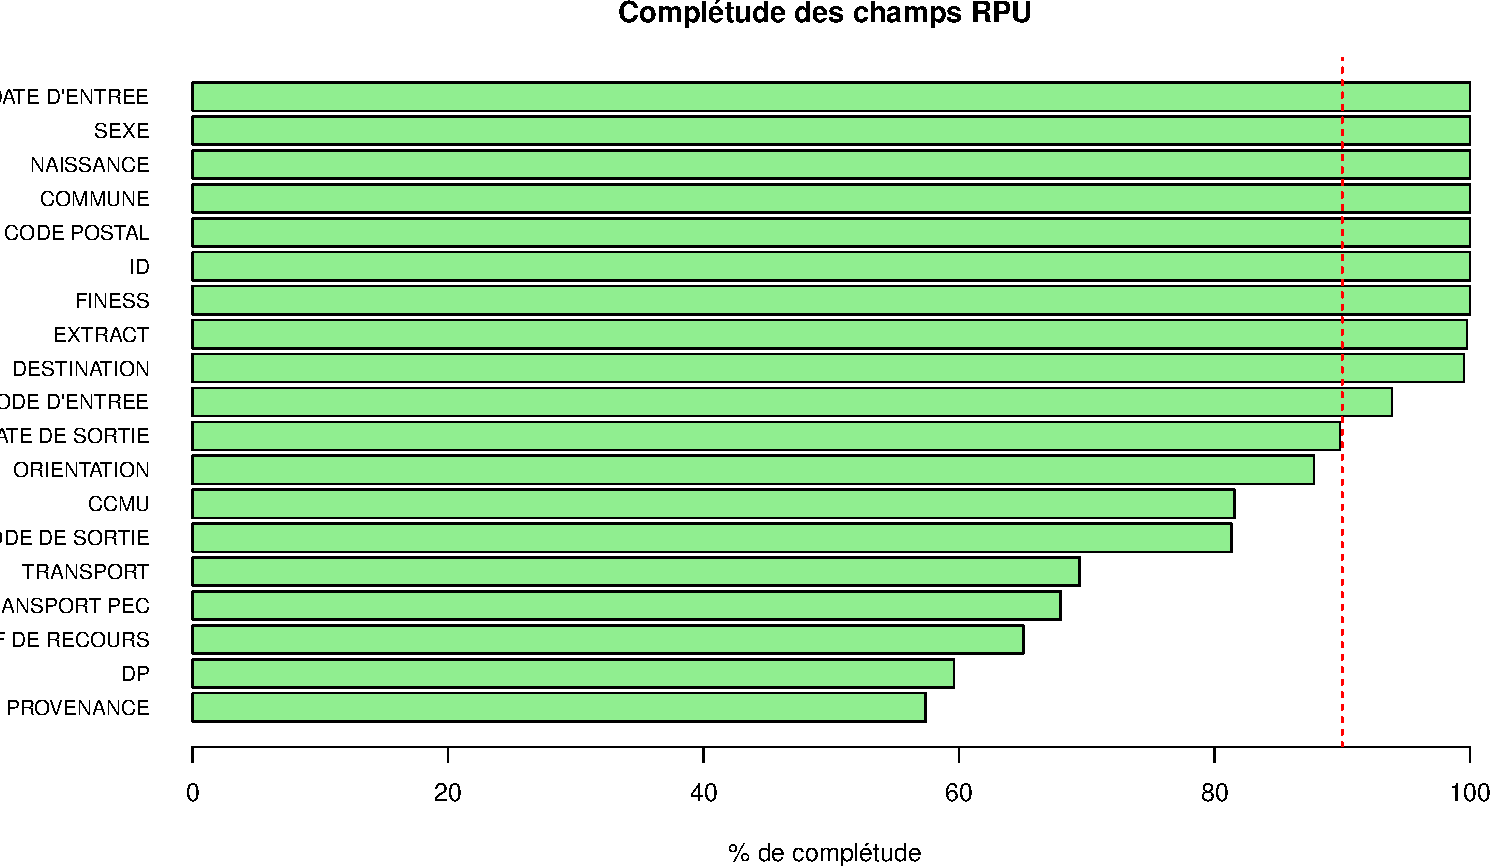
\includegraphics{rapport2014_V4_files/figure-latex/completude-1.pdf}

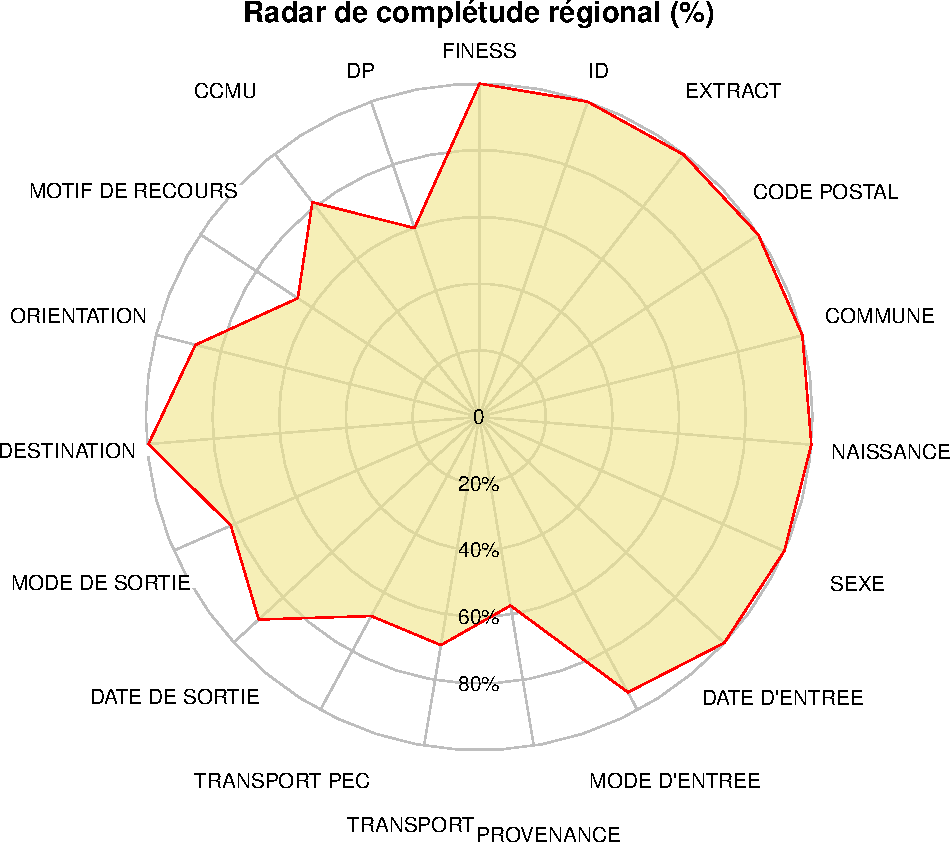
\includegraphics{rapport2014_V4_files/figure-latex/radar-1.pdf}

Complétude en valeur absolue (voir table):

\begin{table}[ht]
\centering
\begin{tabular}{rrr}
  \hline
 & Fréquence & \% exhaustivité \\ 
  \hline
FINESS & 416 733,00 & 100,00 \\ 
  ID & 416 733,00 & 100,00 \\ 
  EXTRACT & 415 731,00 & 99,76 \\ 
  CODE POSTAL & 416 733,00 & 100,00 \\ 
  COMMUNE & 416 716,00 & 100,00 \\ 
  NAISSANCE & 416 733,00 & 100,00 \\ 
  SEXE & 416 733,00 & 100,00 \\ 
  DATE D'ENTREE & 416 733,00 & 100,00 \\ 
  MODE D'ENTREE & 391 370,00 & 93,91 \\ 
  PROVENANCE & 239 122,00 & 57,38 \\ 
  TRANSPORT & 289 308,00 & 69,42 \\ 
  TRANSPORT PEC & 283 189,00 & 67,95 \\ 
  DATE DE SORTIE & 374 349,00 & 89,83 \\ 
  MODE DE SORTIE & 338 878,00 & 81,32 \\ 
  DESTINATION & 82 635,00 & 99,53 \\ 
  ORIENTATION & 72 898,00 & 87,80 \\ 
  MOTIF DE RECOURS & 270 962,00 & 65,02 \\ 
  CCMU & 339 827,00 & 81,55 \\ 
  DP & 245 974,00 & 59,87 \\ 
   \hline
\end{tabular}
\caption{Exhaustivité des RPU alsaciens en 2014} 
\end{table}

\section{Le contexte régional}\label{le-contexte-regional}

\subsection{Démographie régionale}\label{demographie-regionale}

Avec 8280 km², l'Alsace est la plus petite des régions de la France
métropolitaine, mais elle fait partie des plus densément peuplée (225
hab./km²) derrière l'Ile de Fance et le Nord.

Elle comprend deux départements, le Bas-Rhin (67) et le Haut-Rhin (68).
Elle fait partie de la région du Rhin supérieur avec comme le land du
Bade-Wurtemberg et le canton suisse de Bâle avec qui elle partage une
frontière commune.

Au 1er janvier 2012, l'Alsace compte 1 859 869 habitants.

Sur la période 1982-2011, la population régionale a augmenté de 286 300
habitants, soit une croissance annuelle moyenne de quelque 10 000
personnes. Ce dynamisme démographique est avant tout lié à l'excédent
des naissances sur les décès. En trente ans, ce solde naturel contribue
à hauteur de 80 \% à la hausse totale de la population.

Sources:

\begin{itemize}
\itemsep1pt\parskip0pt\parsep0pt
\item
  \href{http://www.insee.fr/fr/ppp/bases-de-donnees/recensement/populations-legales/france-regions.asp?annee=2012}{INSEE
  Recensement}).
\item
  \href{http://www.insee.fr/fr/regions/alsace/default.asp?page=faitsetchiffres/presentation/presentation.htm}{INSEE
  Régions}
\item
  \href{http://www.insee.fr/fr/themes/document.asp?ref_id=20665}{INSEE
  Thèmes}
\end{itemize}

\subsection{Découpage de la région en territoires de
santé}\label{decoupage-de-la-region-en-territoires-de-sante}

La loi Hôpital Patients Santé et territoires (HPST) prévoit le découpage
de chaque région en ``territoires de santé'' (article L1434-11 du code
de la santé publique).

L'Alsace est découpée, du nord au sud, en 4 territoires de santé:

\begin{itemize}
\itemsep1pt\parskip0pt\parsep0pt
\item
  Le territoire 1 (Haguenau)
\item
  Le territoire 2 (Strasbourg)
\item
  Le territoire 3 (Colmar)
\item
  Le territoire 4 (Mulhouse)
\end{itemize}

\begin{center}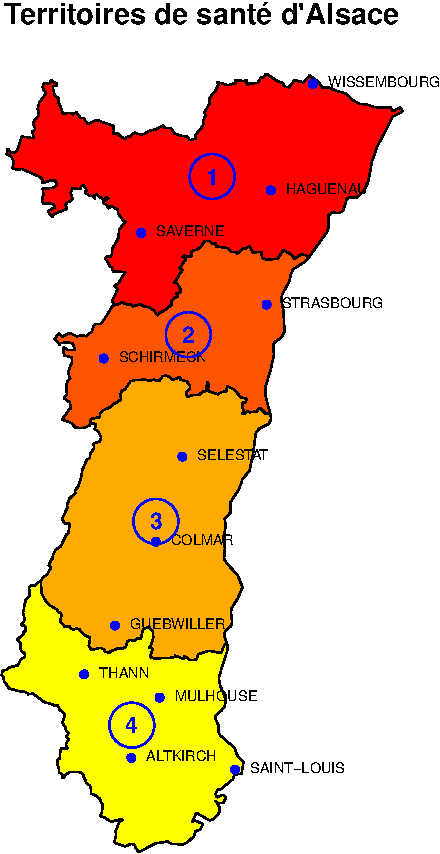
\includegraphics{Figs/unnamed-chunk-43-1} \end{center}

Population 2014:

\begin{table}[ht]
\centering
\begin{tabular}{rlrr}
  \hline
 & Territoire & Population & \% \\ 
  \hline
1 & TERRITOIRE DE SANTE 1 & 358 060 & 19,25 \\ 
  2 & TERRITOIRE DE SANTE 2 & 638 816 & 34,35 \\ 
  3 & TERRITOIRE DE SANTE 3 & 379 681 & 20,41 \\ 
  4 & TERRITOIRE DE SANTE 4 & 483 312 & 25,99 \\ 
   \hline
\end{tabular}
\end{table}

\subsection{Offre de soins régionale}\label{offre-de-soins-regionale}

La région Alsace dispose de 31 structures d'urgence (SU) qui se
répartissent en:

\begin{itemize}
\itemsep1pt\parskip0pt\parsep0pt
\item
  19 services d'urgence polyvalents
\item
  1 structure d'urgence pédiatrique
\item
  2 SAMU
\item
  7 SMUR
\item
  2 hélismur
\end{itemize}

\subsubsection{Etablissements d'Alsace ayant une autorisation de
structure
d'urgence}\label{etablissements-dalsace-ayant-une-autorisation-de-structure-durgence}

Sites gégraphiques d'accueil des urgences:

\begin{itemize}
\item
  Territoire de santé 1

\begin{verbatim}
- CH de Wissembourg (SU polyvalent + SMUR)
- CH de Haguenau (SU polyvalent + SMUR)
- CH de Saverne  (SU polyvalent + SMUR)
\end{verbatim}
\item
  Territoire de santé 2

\begin{verbatim}
- CHU de Strasbourg
- NHC (SU adulte)
- Hôpital de Hautepierre (SU adulte + SU pédiatrique)
- Pôle logistique (SAMU + SMUR + Hélismur)
- Clinique Sainte Odile (SU polyvalent)
- Clinique Sainte Anne (SU polyvalent)
- Clinique du Diaconat (SU Mains)
\end{verbatim}
\item
  Territoire de santé 3

\begin{verbatim}
- CH de Sélestat (SU polyvalent + SMUR)
- CH de Colmar 
- Hôpital Pasteur (SU polyvalent + SMUR)
- Hôpital du parc (SU pédiatrique)
- CH de Guebwiller (SU polyvalent)
\end{verbatim}
\item
  Territoire de santé 4

\begin{verbatim}
- CH de Thann (SU polyvalent)
- CH d'Altkirch (SU polyvalent)
- CH de Mulhouse
- Hôpital Emile Muller (SU polyvalent + SAMU + SMUR + Hélismur)
- Hôpital du Hasenrain (SU pédiatrique)
- Clinique des 3 frontières (SU polyvalent)
- Clinique du Diaconat-Fonderie (SU polyvalent)
- Clinique du Diaconat-Roosvelt (SU Mains)
\end{verbatim}
\end{itemize}

En 2014 tous ces établissements ont fourni des RPU sauf le CH THANN.

\subsection{Cartographie de l'offre de soins
d'urgence}\label{cartographie-de-loffre-de-soins-durgence}

\begin{center}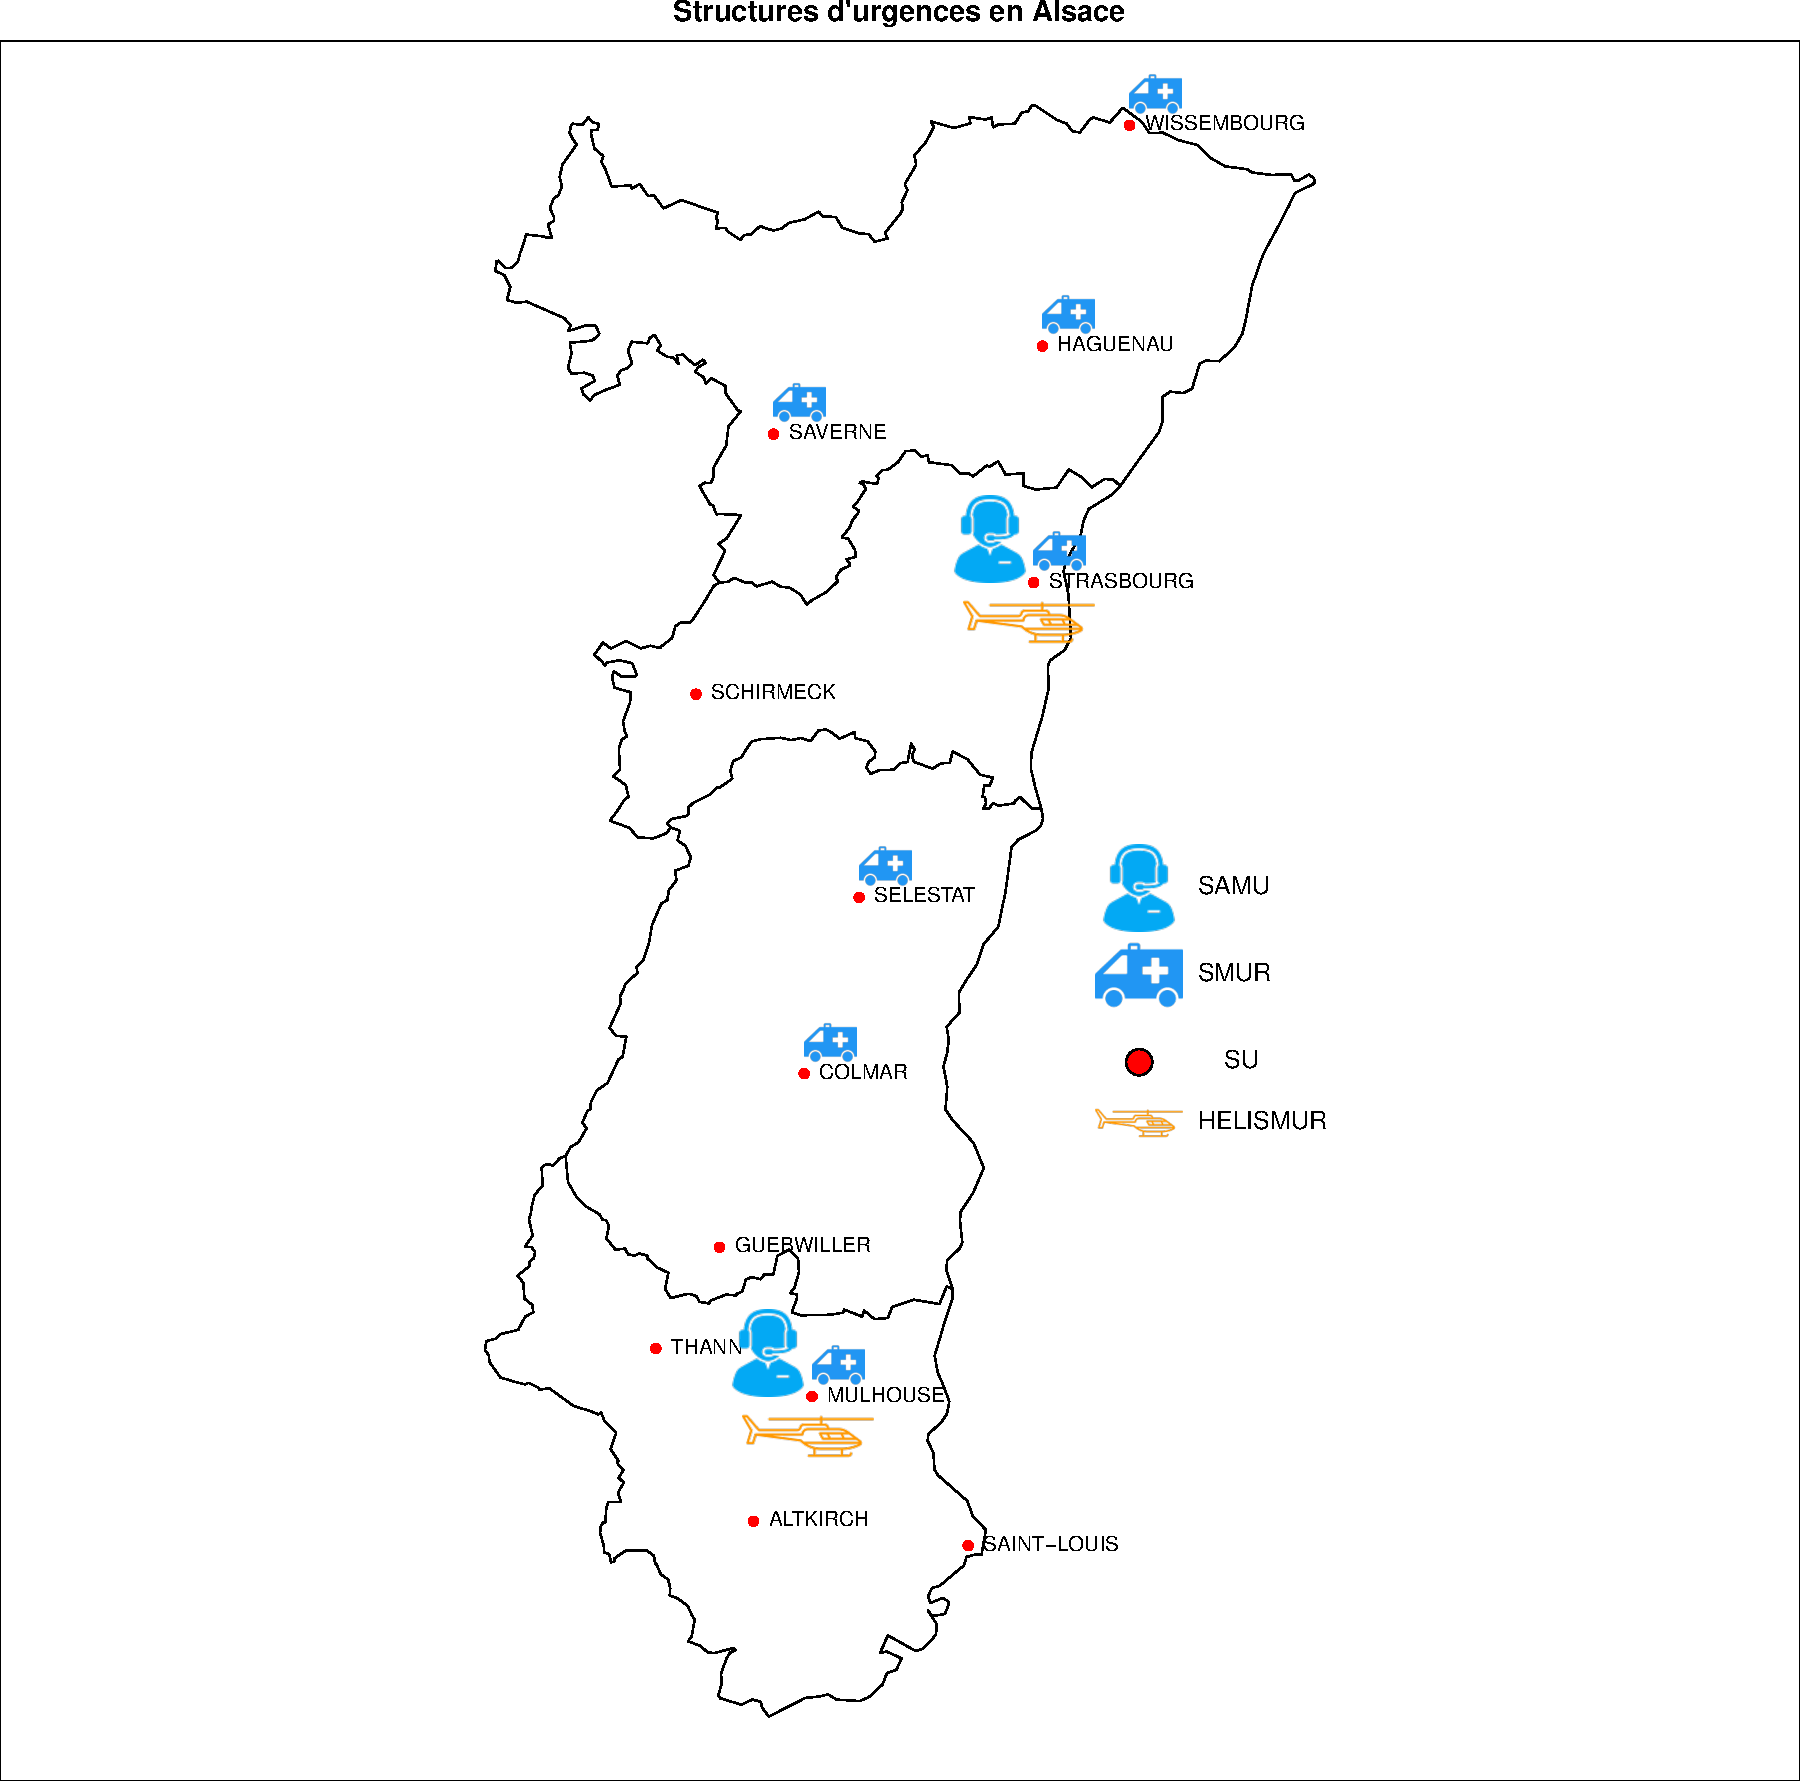
\includegraphics{Figs/samu_smur_su-1} \end{center}

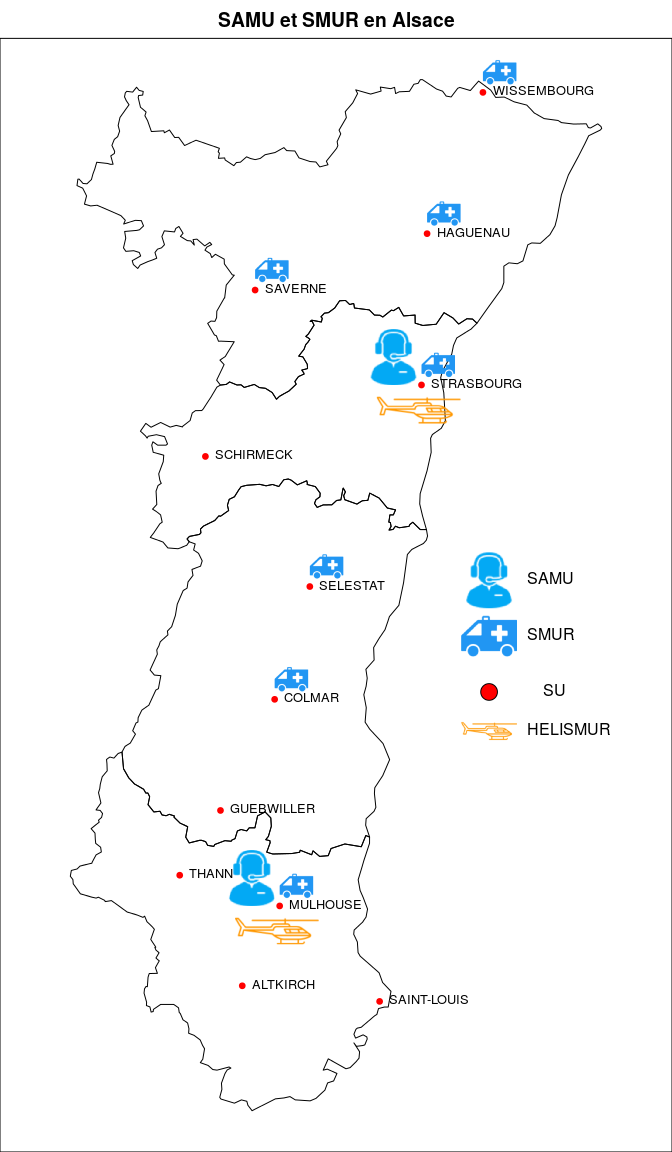
\includegraphics{3-Contexte/Figs/samu_smur_su.png}

\section{Les chiffres clés de l'activité des services
d'urgences}\label{les-chiffres-cles-de-lactivite-des-services-durgences}

Le format des chiffres clés est celui défini par la FEDORU. Il est
commun à toutes les régions membres de la FEDORU.

\subsection{Recueil des données}\label{recueil-des-donnees}

\begin{itemize}
\itemsep1pt\parskip0pt\parsep0pt
\item
  Population alsacienne au 1er janvier 2014: 1 868 773 \href{}{INSEE}
\item
  Nombre de passages dans l'année: 521 129 (données SAE 2014)
\item
  Nombre de passages pour 10.000 habitants: 2 789
\item
  Nombre de RPU déclarés: \textbf{416 733 RPU}
\item
  Nombre de RPU pour 10.000 habitants: 2 230
\item
  Exhaustivité du recueil: \textbf{79.97 \%}
\item
  Moyenne quotidienne de passages: \textbf{1 142 RPU/jour}
\item
  \%(N) d'évolution par rapport à année 2013: \textbf{22 \%}.
\item
  \% d'évolution moyenne sur les 5 dernières années (méthode calcul :
  \emph{pas de données disponibles}.
\item
  Données renseignées (données à partir desquelles tout le reste de
  l'analyse sera effectuée) = Nombre de RPU transmis: 416 733 RPU
\end{itemize}

\subsection{Patients}\label{patients}

\subsubsection{Sexe}\label{sexe}

\begin{itemize}
\itemsep1pt\parskip0pt\parsep0pt
\item
  \%(N) Femme: 47.78 \% (217 617)
\item
  \%(N) Homme: 52.22 \% (199 110)
\item
  Sex ratio: \textbf{1.09}
\item
  Taux de masculinité: 0.52
\end{itemize}

\subsubsection{Age}\label{age}

\begin{itemize}
\item
  age moyen: \textbf{38 ans}.
\item
  age moyen des hommes: 35.9 ans.
\item
  age moyen des femmes: 40.3 ans.
\item
  \% (N) \textless{} 1 an: 15 376 (\textbf{3.69 \%})
\item
  \%(N) \textless{} 15 ans: 103 413 (\textbf{24.82 \%})
\item
  \%(N) \textless{} 18 ans: 119 213 (\textbf{28.61 \%})
\item
  \%(N) \textgreater{}= 75 ans: 57 271 (\textbf{13.74 \%})
\item
  Pyramide des ages:
\end{itemize}

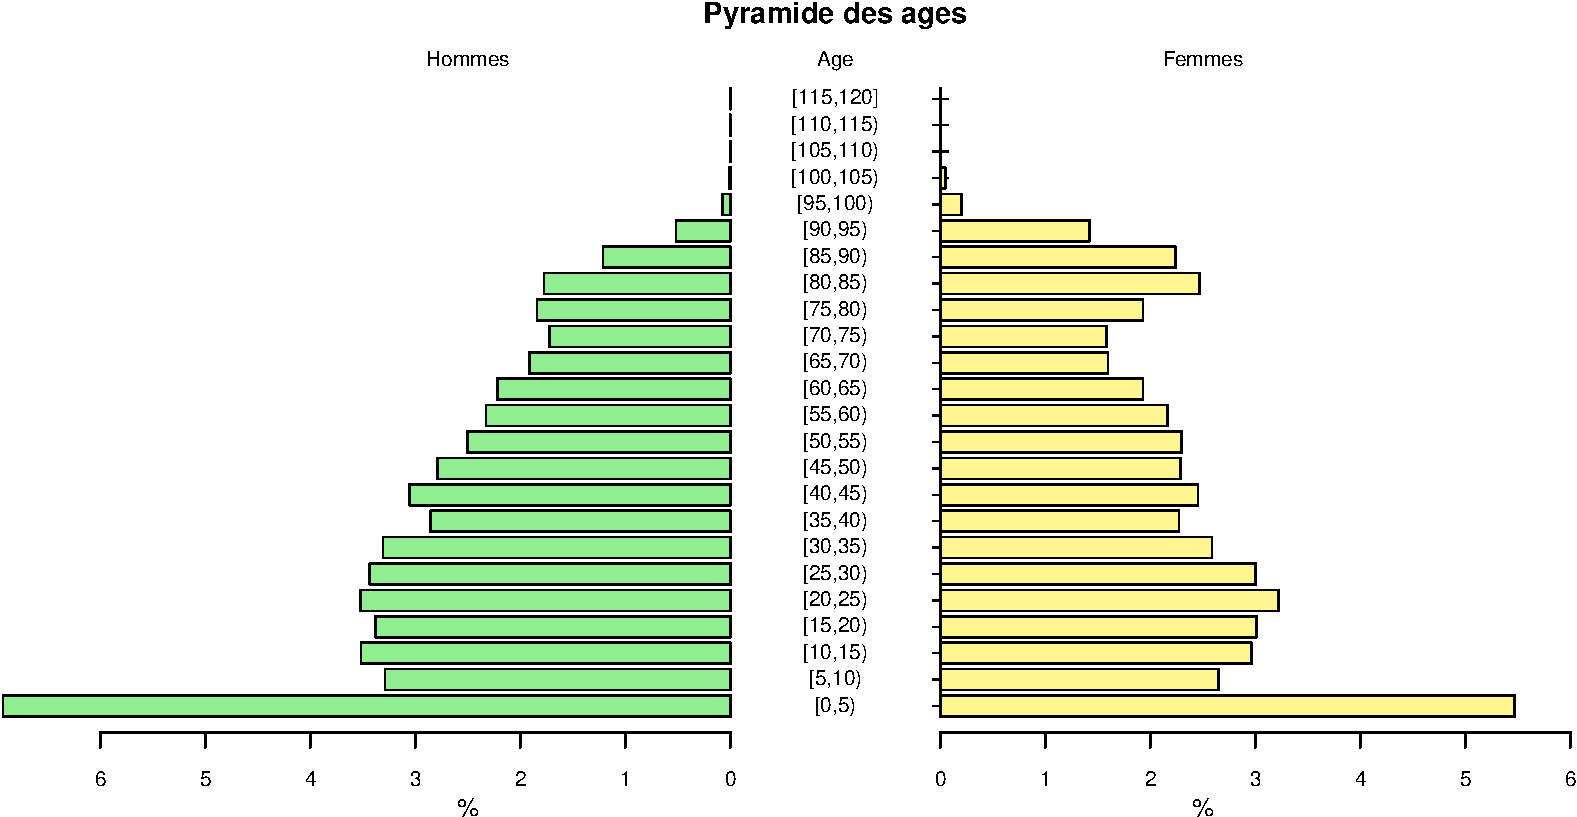
\includegraphics{Figs/pyramide-1.pdf}

\subsubsection{Taux de recours (définition FEDORU) régional aux
urgences.}\label{taux-de-recours-definition-fedoru-regional-aux-urgences.}

Le taux de recours régional est calculé à partir des données de l'INSEE.

TARRU: \textbf{21.31\%} (ref: population alsacienne 2014)

\subsubsection{Pourcentage de Patients ne venant pas de la région
(étranger
compris)}\label{pourcentage-de-patients-ne-venant-pas-de-la-region-etranger-compris}

Part des non résidents: \textbf{4.43\%} (N = 18 467)

\subsection{ARRIVÉE}\label{arrivee}

\subsubsection{Horaires de passage}\label{horaires-de-passage}

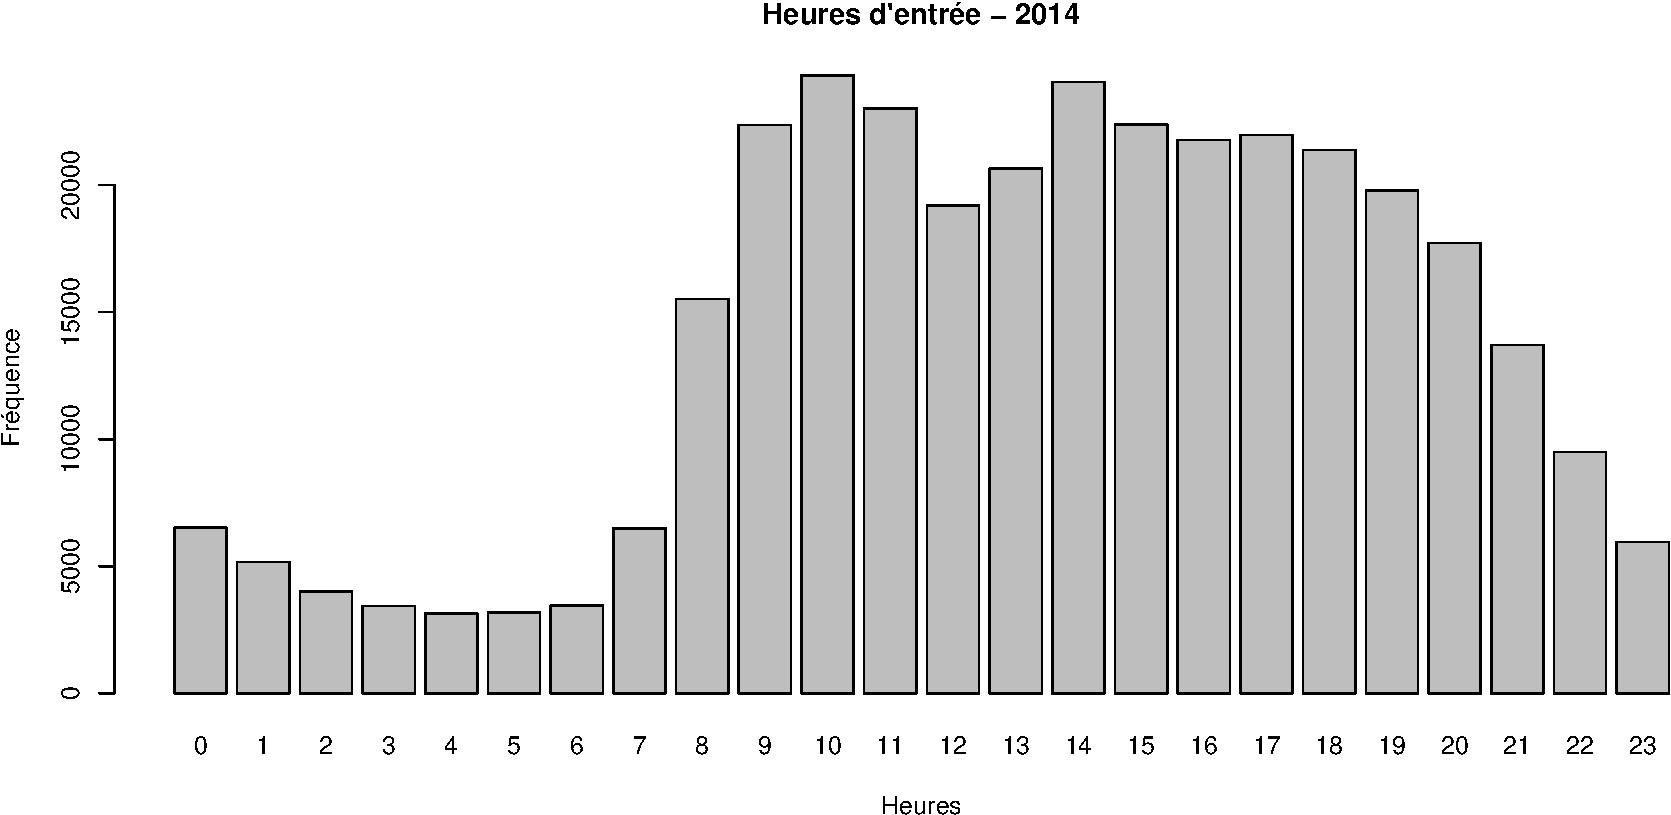
\includegraphics{Figs/horaires-1.pdf}
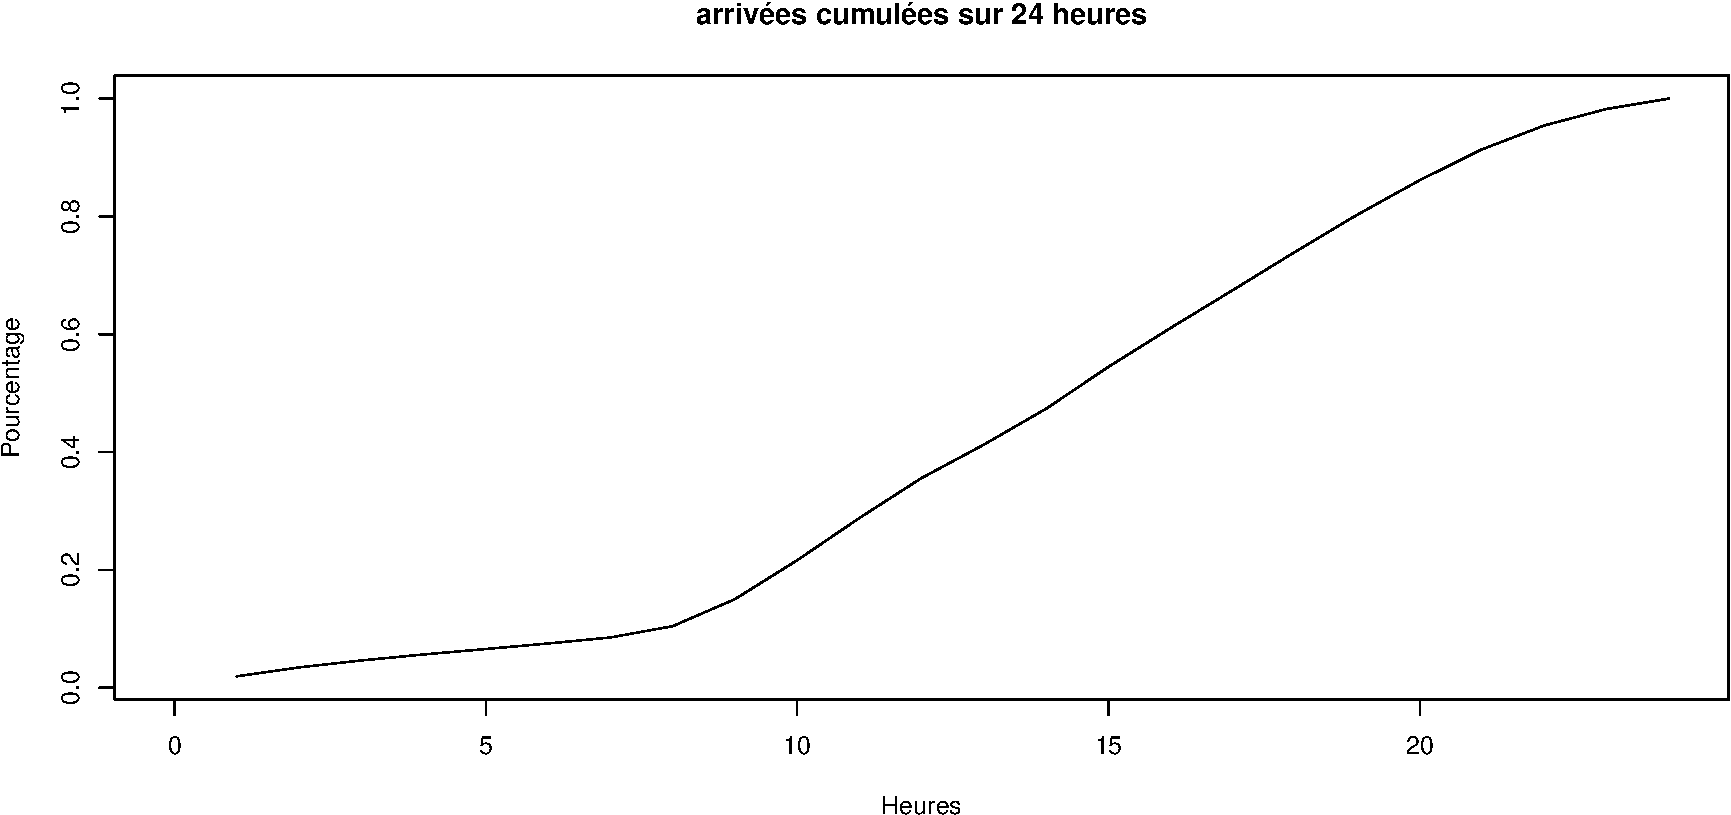
\includegraphics{Figs/horaires-2.pdf}

\begin{itemize}
\item
  Passages de nuit (20h - 8h): \textbf{27.7 \%} (N = 115 418)
\item
  Passages en nuit profonde (0h - 8h): \textbf{10.38 \%} (N = 43 271)
\item
  Passages en horaire de PDSA: \textbf{45.22 \%} N = 188 454 (Remarque:
  ne tient pas compte des jours fériés survenant en semaine)
\end{itemize}

\subsubsection{Variations saisonnières}\label{variations-saisonnieres}

Variation du nombre de RPU entre les mois d'été (juillet-août) et les
autres mois de l'année: \textbf{-5.82 \%}.

\subsubsection{Moyens d'arrivée}\label{moyens-darrivee}

\begin{itemize}
\itemsep1pt\parskip0pt\parsep0pt
\item
  \%(N) moyens de reansport renseignés: \textbf{69.42 \%} (N = 289 308)
\item
  \%(N) d'arrivée personnel: \textbf{72.16 \%} (N = 208 771)
\item
  \%(N) d'arrivée SMUR: \textbf{0.93 \%} (N = 2 702)
\item
  \%(N) d'arrivée VSAB: \textbf{10.35 \%} (N = 29 954)
\item
  \%(N) d'arrivée Ambulance: \textbf{15.94 \%} (N = 46 112)
\end{itemize}

NB : commentaire possible pour expliquer que la somme des 4 pourcentages
ci dessus ne fait pas 100 \%

\subsubsection{Gravité (CCMU)}\label{gravite-ccmu}

\begin{itemize}
\itemsep1pt\parskip0pt\parsep0pt
\item
  nombre de CCMU renseignés: 339 827.
\item
  \%(N) CCMU 1: \textbf{15.21\%} (n = 51 682)
\item
  \%(N) CCMU 1 et 2: \textbf{84.45\%} (n = 286 979)
\item
  \%(N) CCMU 4 et 5: \textbf{1.28\%} (n = 4 341)
\end{itemize}

Exhaustivité CCMU :

\begin{itemize}
\itemsep1pt\parskip0pt\parsep0pt
\item
  Nombre de RPU 2014 hors orientation = FUGUE, PSA et REO ayant un
  élément transmis pour la CCMU: \textbf{335 889}.
\end{itemize}

\subsubsection{Diagnostic principal}\label{diagnostic-principal}

Les diagnostics principaux sont regroupés selon la méthode préconisée
par la FEDORU.

\begin{itemize}
\item
  \% Médico-chirurgical: \textbf{55.35 \%} dont :

  \begin{itemize}
  \itemsep1pt\parskip0pt\parsep0pt
  \item
    \% cardio vasculaire: \textbf{8.33 \%}
  \item
    \% neuro: \textbf{7.9 \%}
  \item
    \% digestif: \textbf{18.93 \%}
  \item
    \% respiratoire: \textbf{9.38 \%}
  \end{itemize}
\item
  \% Traumatologique: \textbf{37.18 \%}
\item
  \% Psychiatrique: \textbf{2.5 \%}
\item
  \% Toxicologique: \textbf{1.96 \%}
\item
  \% Autres recours: \textbf{3.01 \%}
\end{itemize}

\subsubsection{Durées de passage}\label{durees-de-passage}

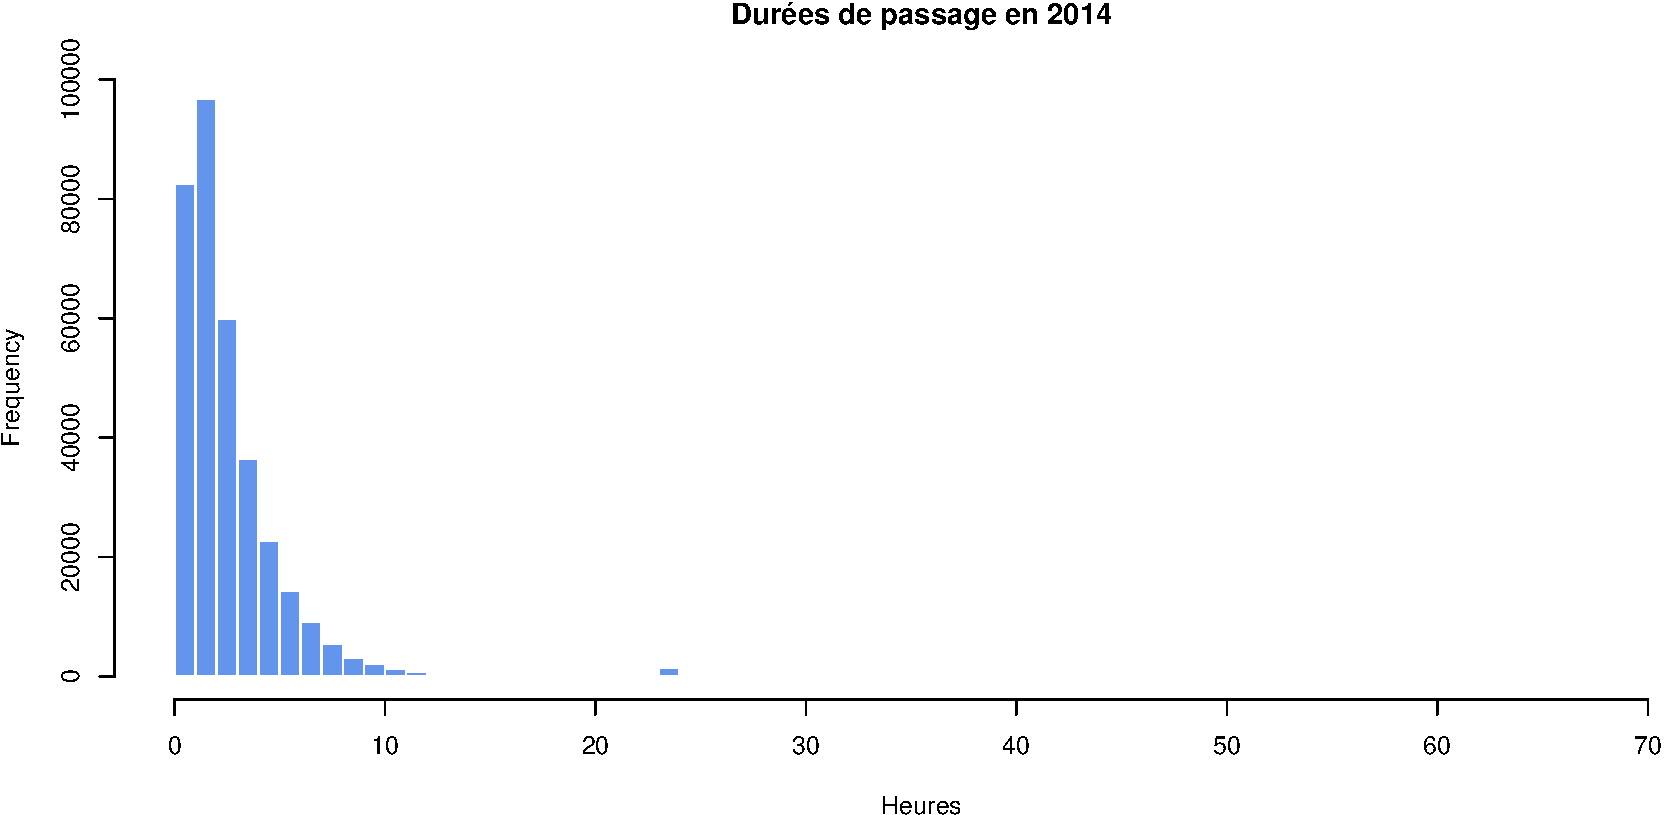
\includegraphics{Figs/passages-1.pdf}

\begin{itemize}
\item
  Nombre de RPU dont la durée de passage est comprise entre 0h et 72h:
  \textbf{338 722}
\item
  durée moyenne de passage \textbf{160 mn} (2h40).
\item
  écart-type: 173.22 mn (2h53).
\item
  médiane: \textbf{113 mn} (1h53).
\item
  nombre de prises en charge \textgreater{} 4 heures: 63 101
  (\textbf{18.63 \%}).
\item
  nombre de prises en charge inférieures ou égales à 4 heures: 275 621
  (\textbf{81.37 \%}).
\item
  Lors d'une hospitalisation post-urgences (hospitalisation = mutation +
  transfert)

  \begin{itemize}
  \itemsep1pt\parskip0pt\parsep0pt
  \item
    moyenne durée de passage en cas d'hospitalisation: \textbf{238.69
    mn}.
  \item
    médiane durée de passage en cas d'hospitalisation: \textbf{198 mn}.
  \end{itemize}
\item
  Lors d'un retour au domicile

  \begin{itemize}
  \itemsep1pt\parskip0pt\parsep0pt
  \item
    moyenne durée de passage en cas de retour à domicile: \textbf{145.66
    mn}.
  \item
    médiane durée de passage en cas de retour à domicile: \textbf{103
    mn}.
  \end{itemize}
\end{itemize}

(source: temps de passages.Rmd)

\subsubsection{Mode de sortie}\label{mode-de-sortie}

\begin{itemize}
\itemsep1pt\parskip0pt\parsep0pt
\item
  \% (N) de retour à domicile: \textbf{75.5 \%} (N = 255 852)
\item
  \% (N) Hospitalisation: \textbf{24.5 \%} (N = 83 024)
\item
  \% (N) Mutation: \textbf{22.72 \%} (N = 76 999)
\item
  \% (N) Transfert: \textbf{1.78 \%} (N = 6 025)
\item
  Nb de RPU 2014 avec mode de sortie = 6 ou 7 (hospitalisation)
  \textbf{avec} un élément transmis pour la destination: \textbf{82 635}
\item
  Nb de RPU 2014 avec mode de sortie = 6 ou 7 \textbf{avec} un élement
  transmis pour l'orientation: \textbf{72 898}
\end{itemize}

\section{Les chiffres clés de l'activité des
SAMU}\label{les-chiffres-cles-de-lactivite-des-samu}

(à partir des données SRVA ``officielles'')

\begin{itemize}
\itemsep1pt\parskip0pt\parsep0pt
\item
  Nombre de dossiers de régulation médicale (DRM): 480 303
\item
  Nombre de SMUR : 25 321

  \begin{itemize}
  \itemsep1pt\parskip0pt\parsep0pt
  \item
    dont primaires: 19 714
  \end{itemize}
\item
  Nombre d'ambulances privées à la demande du SAMU: 46 031
\end{itemize}

\subsection{Organisation}\label{organisation}

\subsubsection{Nombre de colonnes SMUR
terrestres:}\label{nombre-de-colonnes-smur-terrestres}

\begin{longtable}[c]{@{}lll@{}}
\toprule
SMUR & Jour & Nuit\tabularnewline
\midrule
\endhead
Wissembourg & 1 & 1\tabularnewline
Haguenau & 1 & 1\tabularnewline
Saverne & 1 & 1\tabularnewline
Strasbourg & 4 & 3\tabularnewline
Sélestat & 1 & 1\tabularnewline
Colmar & 2 & 2\tabularnewline
Mulhouse & 2 & 2\tabularnewline
\bottomrule
\end{longtable}

\subsubsection{Nombre de SMUR
héliportés:}\label{nombre-de-smur-heliportes}

\begin{longtable}[c]{@{}llll@{}}
\toprule
SMUR & Jour & Nuit & Remarques\tabularnewline
\midrule
\endhead
Strasbourg & 1 & 1 & convention avec la sécurité civile\tabularnewline
Mulhouse & 1 & 1 & colonne mutualisée avec le SMUR
terrestre\tabularnewline
\bottomrule
\end{longtable}

\subsubsection{Nombre de SMUR
pédiatriques:}\label{nombre-de-smur-pediatriques}

\begin{longtable}[c]{@{}lll@{}}
\toprule
SMUR & Jour & Nuit\tabularnewline
\midrule
\endhead
Strasbourg (HTP) & 1 & 1\tabularnewline
\bottomrule
\end{longtable}

\subsubsection{SAMU}\label{samu}

\begin{itemize}
\itemsep1pt\parskip0pt\parsep0pt
\item
  Nombre de SAMU: 2
\item
  Nombre de SAMU par bassin populationnel (pour 100 000): 0.11
\item
  Nombre de dossier de régulation médicale pour 100.000 h: 25 702
\item
  Nombre de lignes SMUR par bassin populationnel (pour 100 000): 0.7
\item
  Nombre de SU géographiques par bassin populationnel (pour 100 000):
  1.02
\end{itemize}

\section{Les chiffres clés de l'activité pédiatrique des services
d'urgences (moins de 18
ans)}\label{les-chiffres-cles-de-lactivite-pediatrique-des-services-durgences-moins-de-18-ans}

\subsection{Recueil des données}\label{recueil-des-donnees-1}

\begin{itemize}
\itemsep1pt\parskip0pt\parsep0pt
\item
  Nombre de passages dans l'année: 119 213
\item
  Moyenne quotidienne de passage: 327 passages/j
\item
  Taux d'urgences pédiatriques {[}(Nb RPU Pédia/ Nb RPU global)x100{]}:
  29 \%
\item
  TODO: \% d'évolution par rapport à l'année N-1(données SAE pour ceux
  qui n'ont pas d'historique RPU fiable et permettant la comparaison,
  préciser l'origine des données)
\end{itemize}

\subsection{Patients}\label{patients-1}

\subsubsection{Répartition par tranches
d'âge}\label{repartition-par-tranches-dage}

\begin{table}[ht]
\centering
\begin{tabular}{rr}
  \hline
 & ped \\ 
  \hline
$<$28j & 1 791 \\ 
  28j-1an[ & 13 554 \\ 
  1-5ans[ & 36 287 \\ 
  5-10ans[ & 24 738 \\ 
  10-15ans[ & 27 012 \\ 
  15-18ans[ & 15 800 \\ 
   \hline
\end{tabular}
\caption{Nombre de RPU pédiatriques en 2014 par grandes classes d'âge} 
\end{table}

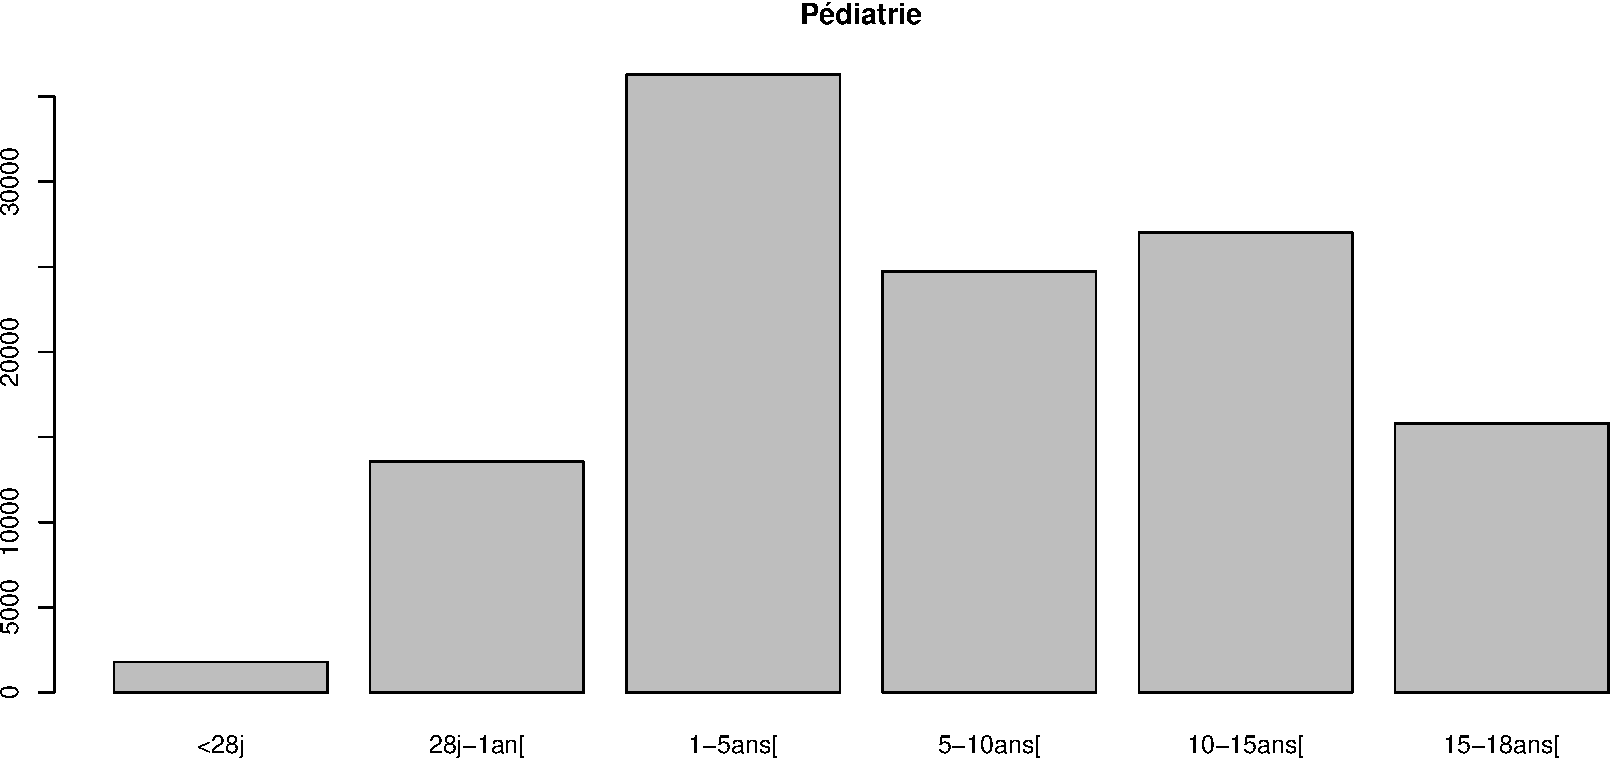
\includegraphics{Figs/unnamed-chunk-7-1.pdf}

\subsubsection{Pyramide des âges}\label{pyramide-des-ages}

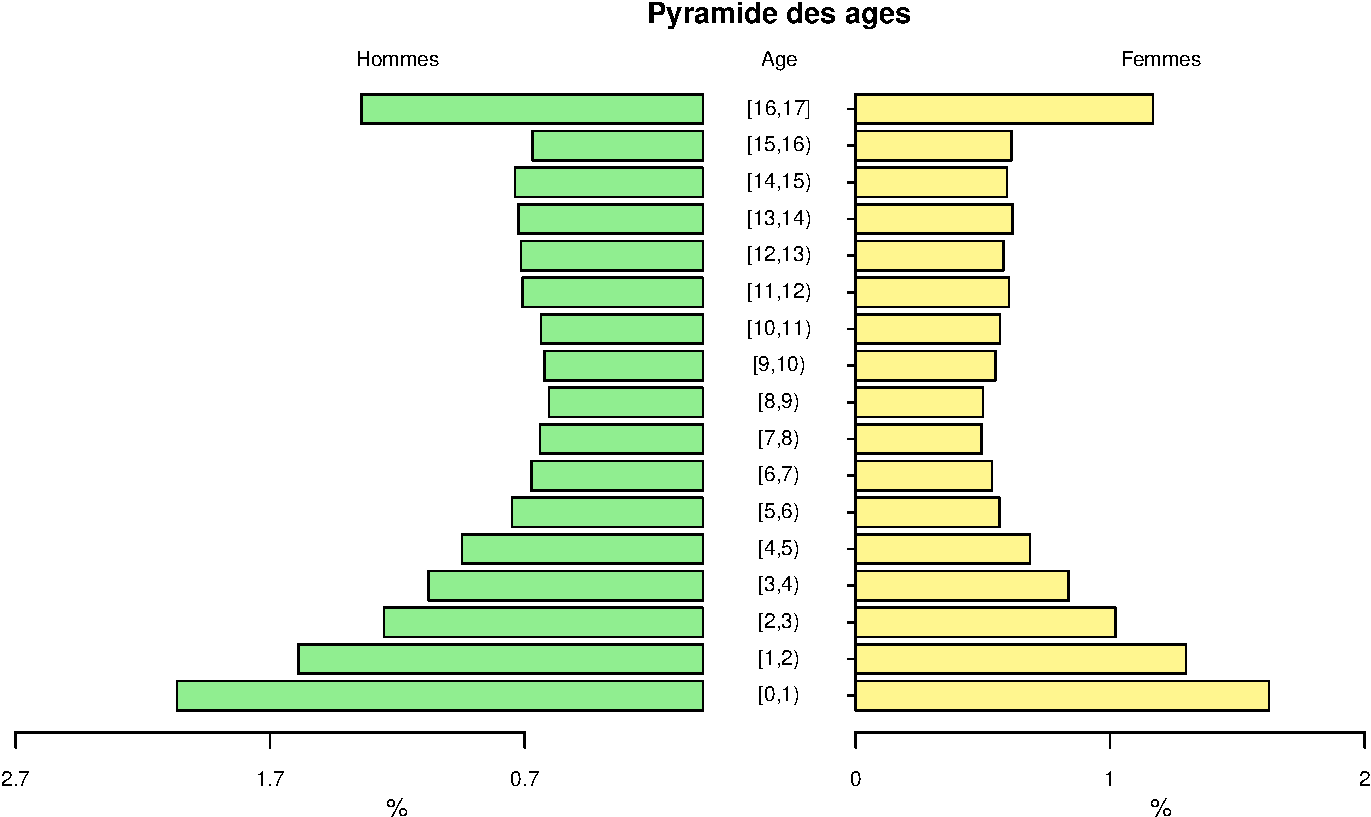
\includegraphics{Figs/unnamed-chunk-8-1.pdf}

\begin{itemize}
\itemsep1pt\parskip0pt\parsep0pt
\item
  nombre de garçons: 65 619
\item
  nombre de filles: 53 590
\item
  Sex ratio: 1.22
\item
  Pyramide des âges (âge par année, borne supérieure toujours exclue)
\item
  Par sous classes d'âge:
\end{itemize}

\subsubsection{mode de transport
pédiatrique}\label{mode-de-transport-pediatrique}

nombre de RPU pédiatriques avec un moyen de transport renseigné: 77 690
(p = 65.17 \%)

\begin{table}[ht]
\centering
\begin{tabular}{rrr}
  \hline
 & Fréq. & \% \\ 
  \hline
AMBU & 2 024,00 & 2,61 \\ 
  FO & 81,00 & 0,10 \\ 
  HELI & 17,00 & 0,02 \\ 
  PERSO & 71 809,00 & 92,43 \\ 
  SMUR & 706,00 & 0,91 \\ 
  VSAB & 3 053,00 & 3,93 \\ 
   \hline
\end{tabular}
\caption{Modes de transports pédiatriques} 
\end{table}

\subsubsection{Gravité des RPU
pédiatriques}\label{gravite-des-rpu-pediatriques}

nombre de CCMU pédiatriques renseignés: 94 706 (p = 79.44 \%)

\begin{table}[ht]
\centering
\begin{tabular}{rrr}
  \hline
 & Fréq. & \% \\ 
  \hline
1 & 24 353,00 & 25,71 \\ 
  2 & 63 361,00 & 66,90 \\ 
  3 & 6 678,00 & 7,05 \\ 
  4 & 211,00 & 0,22 \\ 
  5 & 23,00 & 0,02 \\ 
  D & 2,00 & 0,00 \\ 
  P & 78,00 & 0,08 \\ 
   \hline
\end{tabular}
\caption{Gravité des RPU pédiatriques en 2014.} 
\end{table}

\begin{itemize}
\item
  \% Médico-chirurgical: 51.59 \% dont :

  \begin{itemize}
  \itemsep1pt\parskip0pt\parsep0pt
  \item
    \% cardio vasculaire: \textbf{0.97 \%}
  \item
    \% neuro: \textbf{3.96 \%}
  \item
    \% digestif: \textbf{24.87 \%}
  \item
    \% respiratoire: \textbf{10.19 \%}
  \item
    \% infectieux: \textbf{5.31 \%}
  \end{itemize}
\item
  \% Traumatologique: 44.27 \%
\item
  \% Psychiatrique: 0.94 \%
\item
  \% Toxicologique: 0.71 \%
\item
  \% Autres recours: 2.5 \%
\end{itemize}

\subsubsection{horaires de passages
pédiatriques}\label{horaires-de-passages-pediatriques}

\begin{itemize}
\itemsep1pt\parskip0pt\parsep0pt
\item
  nombre de passages la nuit: 32 677 (p = 27.41 \%)
\item
  nombre de passages en nuit profonde: 8 660 (p = 7.26 \%)
\end{itemize}

\subsubsection{Durée de passage}\label{duree-de-passage}

\begin{itemize}
\item
  Nombre de RPU avec une heure de sortie conforme ({]}0-72h{[}: 106 660
\item
  Durée moyenne de passage (en min): 120.76 mn
\item
  Durée médiane de passage (en min): 86 mn
\item
  Nombre de RPU dont la durée de passage est inférieure à 4h: 99 128
\item
  Nombre de RPU avec une heure de sortie conforme ({]}0-72h{[} lors
  d'une hospitalisation post-urgences: 9 537
\item
  Nombre de RPU avec une heure de sortie conforme ({]}0-72h{[} lors d'un
  retour au domicile: 83 458
\item
  Nombre de RPU dont la durée de passage est inférieure à 4h lors d'une
  hospitalisation post-urgences: 8 532
\item
  Nombre de RPU dont la durée de passage est inférieure à 4h lors d'un
  retour au domicile: 90 595
\item
  Nombre de RPU avec un mode de sortie renseigné: 96 860
\item
  Nombre de mutation interne: 11 996
\item
  Nombre de transfert externe: 556
\item
  nombre de retours à domicile: 84 307
\end{itemize}

\section{Les chiffres clés de l'activité gériatrique des services
d'urgences (75 ans et
plus)}\label{les-chiffres-cles-de-lactivite-geriatrique-des-services-durgences-75-ans-et-plus}

En 2014, l'Alsace recense 155 281 personnes de 75 ans ou plus.

\subsection{Recueil des données}\label{recueil-des-donnees-2}

\begin{itemize}
\itemsep1pt\parskip0pt\parsep0pt
\item
  Nombre de passages dans l'année: \textbf{57 271}
\item
  Taux de recours aux SU de la population gériatrique: \textbf{36.88 \%}
\item
  Moyenne quotidienne de passage: \textbf{157 passages/j}
\item
  Taux d'urgences gériatriques {[}(Nb RPU Géria/ Nb RPU global)x100{]}:
  \textbf{13.74 \%}
\item
  \% d'évolution par rapport à l'année N-1: \emph{données non fiables}.
\end{itemize}

\subsection{Patients}\label{patients-2}

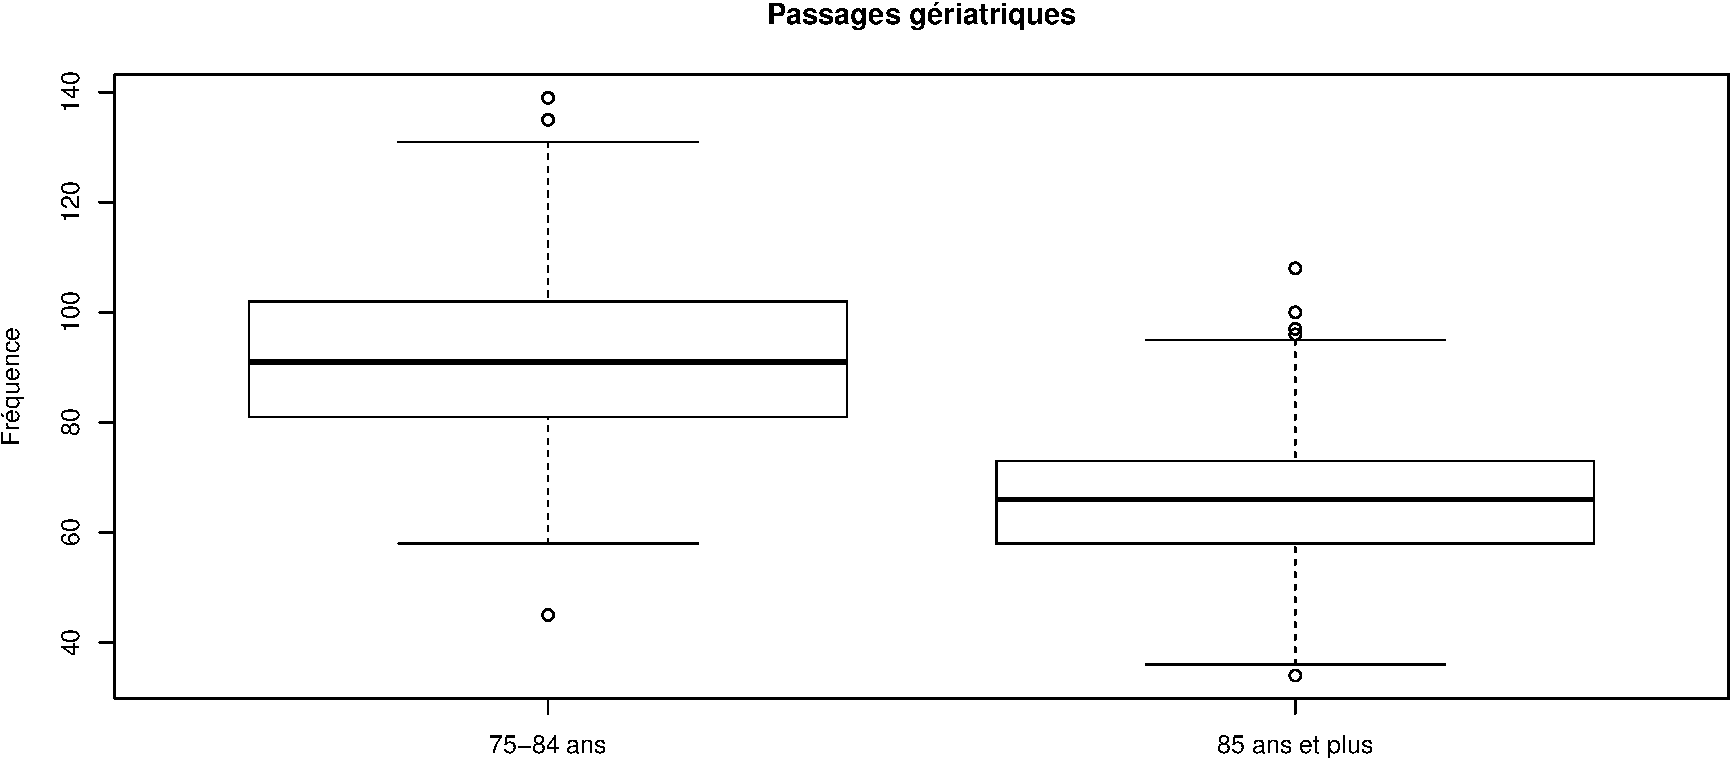
\includegraphics{Figs/sexe75-1.pdf}

\begin{itemize}
\item
  Nombre d'hommes: 22 665
\item
  Nombre de femmes: 34 605
\item
  Sex ratio: 0.65
\item
  Pyramide des âges (âge par année, borne supérieure toujours exclue)
\item
  Par sous classes d'âge (voir \ref{table.synthese.75}):

  \begin{itemize}
  \itemsep1pt\parskip0pt\parsep0pt
  \item
    85 ans ou moins: 33 399
  \item
    plus de 85 ans: 23 872
  \end{itemize}
\end{itemize}

\begin{table}[ht]
\centering
\begin{tabular}{rrrrr}
  \hline
 & effectif & moyenne par jour  & médiane par jour & sex ratio \\ 
  \hline
75-84 ans & 33 399 & 91,50 &  91 & 0,82 \\ 
  85 ans et plus & 23 872 & 65,40 &  66 & 0,47 \\ 
   \hline
\end{tabular}
\caption{Caractéristiques des patients de 75 ans et plus, répartis en deux classes d'âge} 
\end{table}

\subsubsection{Pyramides des ages}\label{pyramides-des-ages}

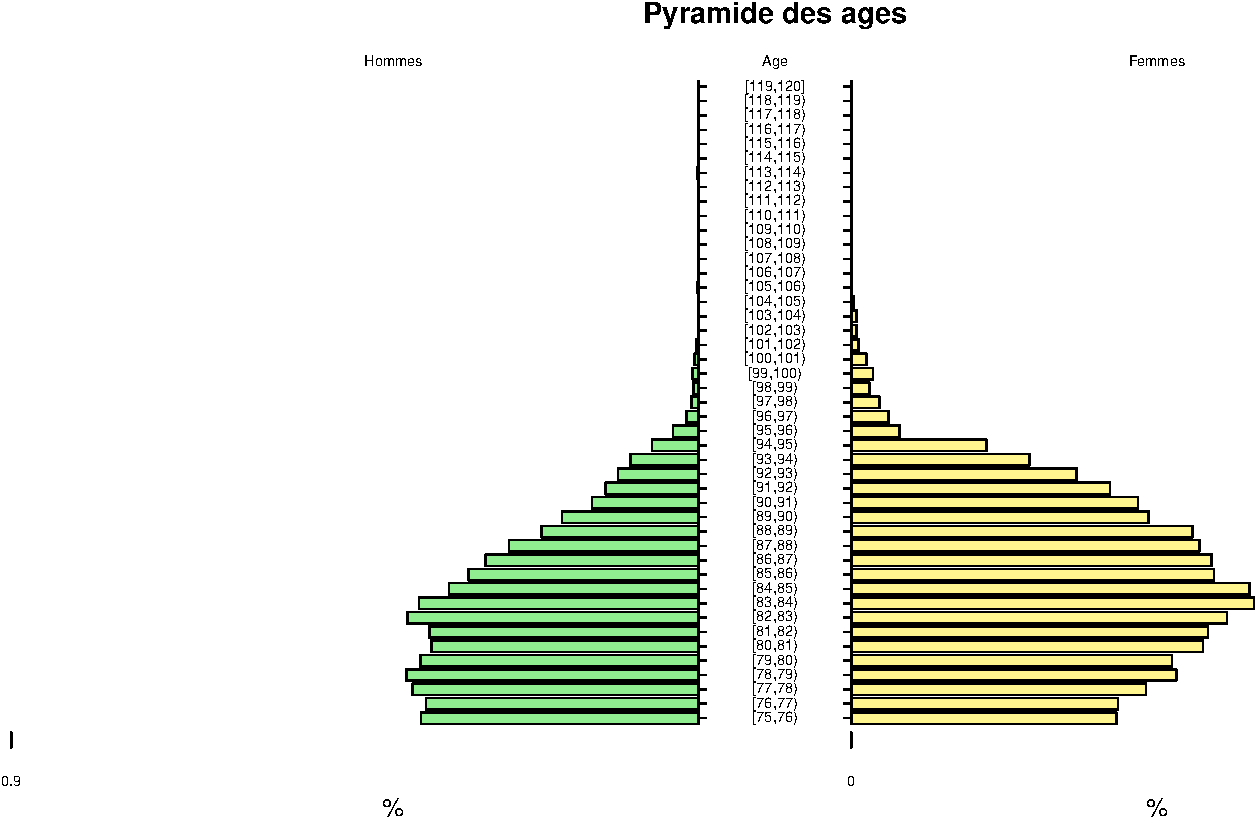
\includegraphics{Figs/unnamed-chunk-11-1.pdf}

\subsection{ARRIVÉE}\label{arrivee-1}

\subsubsection{Horaires de passage}\label{horaires-de-passage-1}

\begin{itemize}
\itemsep1pt\parskip0pt\parsep0pt
\item
  Nb de RPU avec date/heure d'entrée renseignés: \textbf{57 271}
\item
  \% passages la nuit: \textbf{22.38 \%} (N = 12 815)
\item
  \% passages en horaire de PDS: \textbf{38.12 \%} (N = 21 830)
\end{itemize}

\subsubsection{Moyens de transport}\label{moyens-de-transport}

\begin{itemize}
\item
  nombre de moyens de transport: 57 271
\item
  nombre de moyens de transport renseignés: 40 878
\item
  nombre de moyens personnels: 11 962
\item
  nombre de SMUR: 698
\item
  nombre de VSAV: 6 797
\item
  nombre d'ambulances privées: 21 370
\item
  \% d'arrivées Moyen perso: \_\textbf{0.29 \%} (N = 11 962)
\item
  \% d'arrivées SMUR: \textbf{0.17 \%} (N = 6 797)
\item
  \% d'arrivées VSAV: \textbf{0.17 \%} (N = 6 797)
\item
  \% d'arrivées ambulance privée: \textbf{0.52 \%} (N = 21 370)
\item
  \% réponses manquantes: \textbf{28.62 \%}
\end{itemize}

NB : commentaire possible pour expliquer que la somme des 4 pourcentages
ci dessus ne fait pas 100 \%

\subsubsection{Gravité}\label{gravite}

\begin{itemize}
\itemsep1pt\parskip0pt\parsep0pt
\item
  Nombre de RPU avec une CCMU renseignée: 47 408
\item
  \% CCMU 1: \textbf{4.32 \%} (N = 2 472)
\item
  \% CCMU 4 et 5: \textbf{3.14 \%} (N = 1 797)
\end{itemize}

\subsubsection{Diagnostic principal}\label{diagnostic-principal-1}

\begin{itemize}
\item
  \% Médico-chirurgical: 71.51 \%

\begin{verbatim}
- dont :
        - % cardio vasculaire:
        - % neuro:
        - % digestif:
        - % respiratoire:
\end{verbatim}
\item
  \% Traumatologique: 25.03 \%
\item
  \% Psychiatrique: 1.23 \%
\item
  \% Toxicologique: 0.57 \%
\item
  \% Autres recours: 1.66 \%
\end{itemize}

\subsubsection{DURÉE}\label{duree}

\begin{verbatim}
##               Mutation Transfert Domicile
## Durée moyenne      219       316      215
## Durée médiane      200       248      174
\end{verbatim}

\begin{verbatim}
## 
##  Welch Two Sample t-test
## 
## data:  passages75$duree by passages75$DEVENIR
## t = -5, df = 40000, p-value = 0.000002
## alternative hypothesis: true difference in means is not equal to 0
## 95 percent confidence interval:
##  -12.7  -5.3
## sample estimates:
## mean in group Domicile     mean in group Hosp 
##                    215                    224
\end{verbatim}

\begin{verbatim}
## [1] 0.0000016
\end{verbatim}

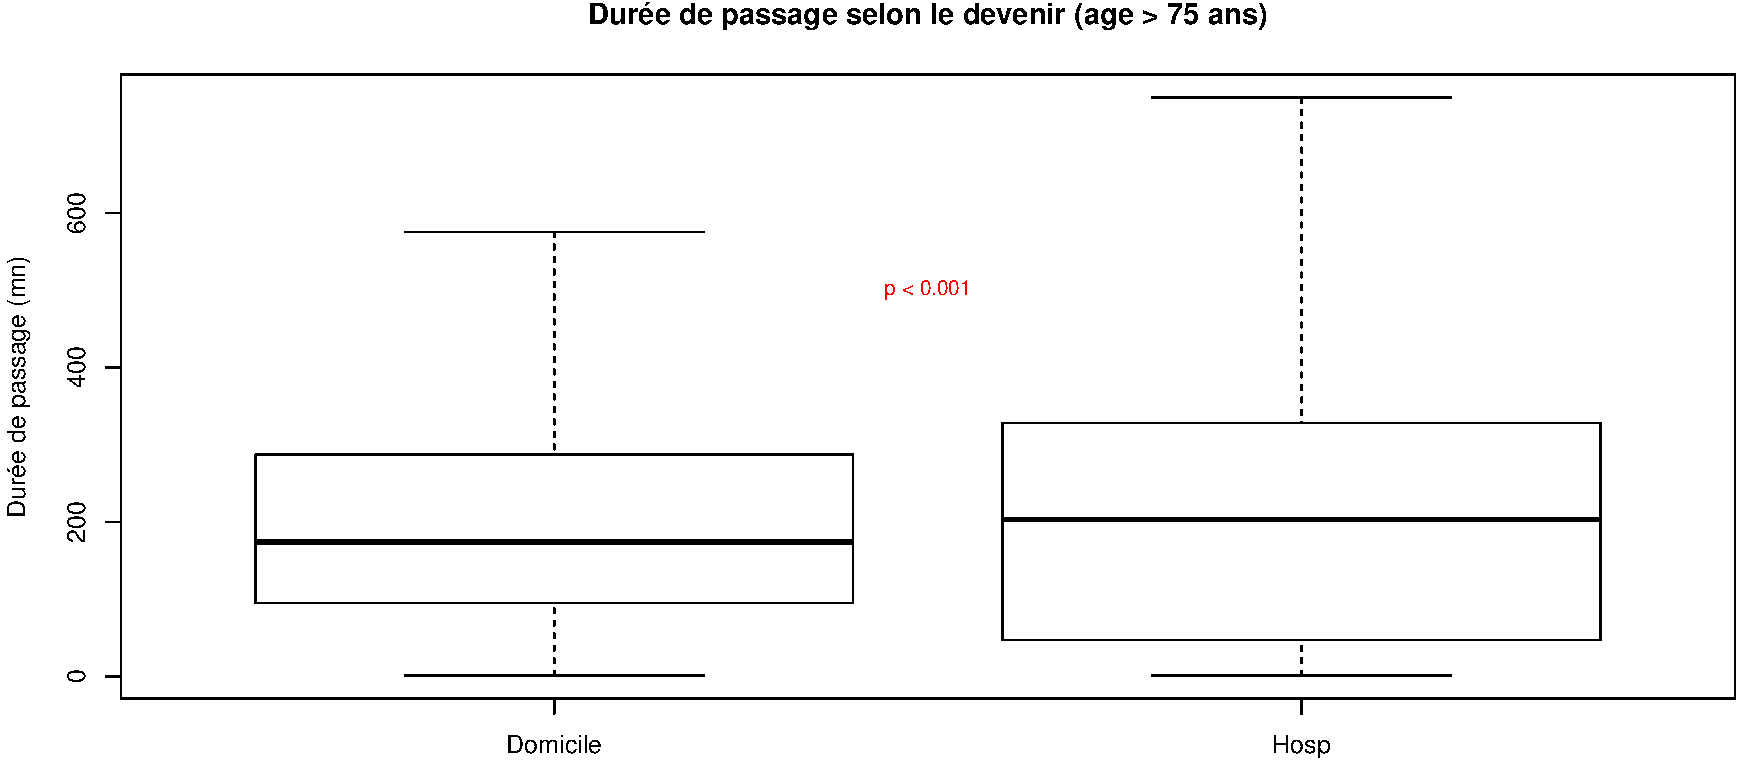
\includegraphics{Figs/duree_passage_75-1.pdf}

\begin{itemize}
\itemsep1pt\parskip0pt\parsep0pt
\item
  Durée moyenne de passage (HORS UHCD) : 220 minutes
\item
  Durée médiane de passage (HORS UHCD) : 190 minutes
\item
  \% de passages de moins de 4h : 61.22 \%
\item
  lors d'une hospitalisation post-urgences (hospitalisation = mutation +
  transfert): 223.7 minutes.
\item
  lors d'un retour au domicile: 214.71 minutes.
\end{itemize}

\paragraph{Nouveau}\label{nouveau}

\begin{itemize}
\item
  Nombre de RPU avec une heure de sortie conforme ({]}0-72h{[}: 37 603
\item
  Durée moyenne de passage (en min): 246.62 mn
\item
  Durée médiane de passage (en min): 210 mn
\item
  Nombre de RPU dont la durée de passage est inférieure à 4h: 21 716
\item
  Nombre de RPU avec une heure de sortie conforme ({]}0-72h{[} lors
  d'une hospitalisation post-urgences: 17 066
\item
  Nombre de RPU avec une heure de sortie conforme ({]}0-72h{[} lors d'un
  retour au domicile: 17 307
\item
  Nombre de RPU dont la durée de passage est inférieure à 4h lors d'une
  hospitalisation post-urgences: 8 109
\item
  Nombre de RPU dont la durée de passage est inférieure à 4h lors d'un
  retour au domicile: 13 607
\end{itemize}

\subsubsection{MODE DE SORTIE}\label{mode-de-sortie-1}

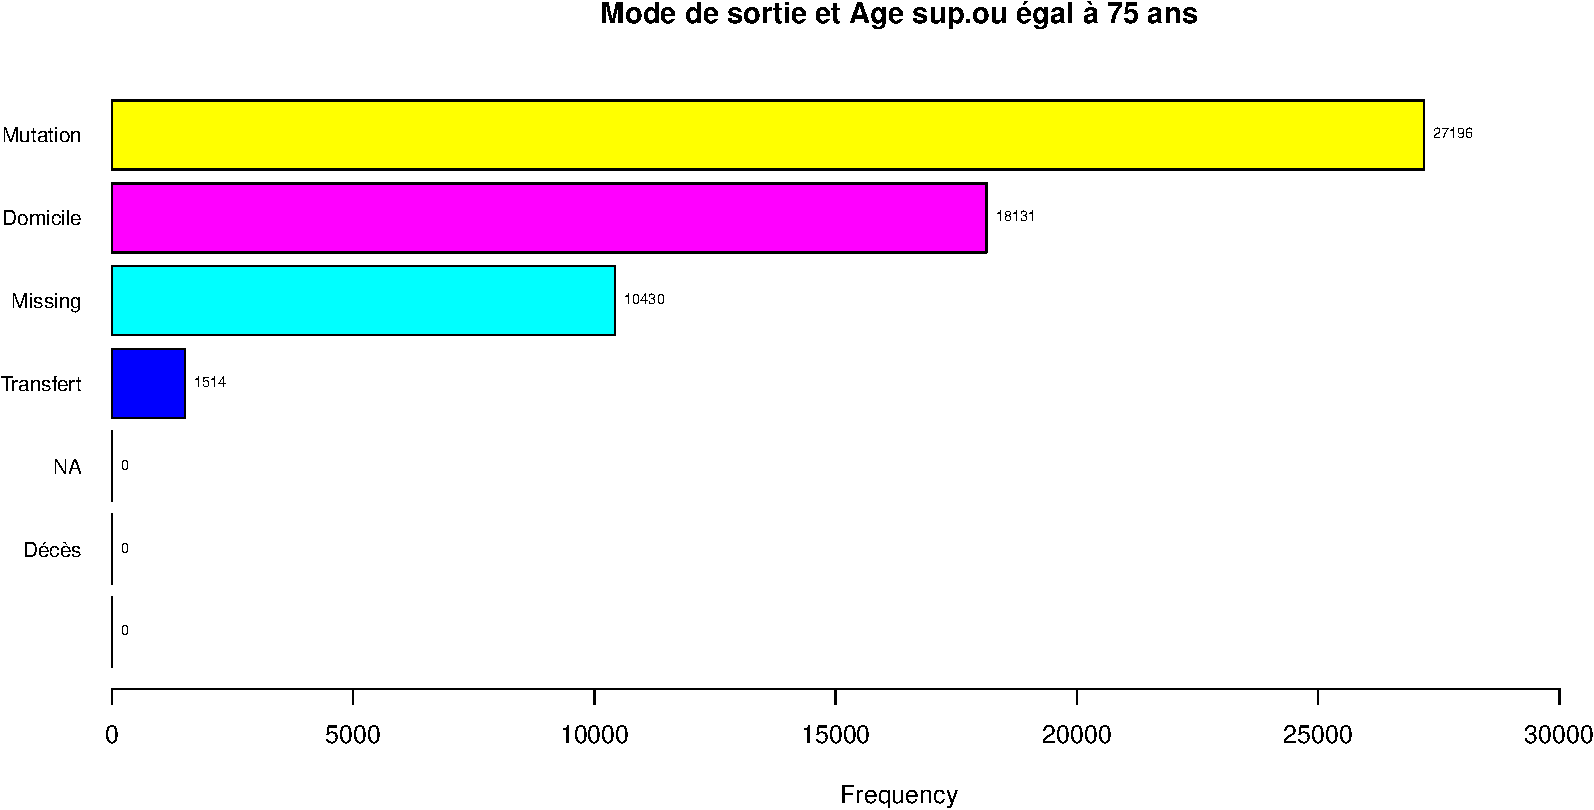
\includegraphics{Figs/sortie75-1.pdf}

\begin{verbatim}
## pop75$MODE_SORTIE : 
##           Frequency   %(NA+)   %(NA-)
## Mutation      27196     47.5     58.1
## Domicile      18131     31.7     38.7
## NA's          10430     18.2      0.0
## Transfert      1514      2.6      3.2
## NA                0      0.0      0.0
## Décès             0      0.0      0.0
##                   0      0.0      0.0
##   Total       57271    100.0    100.0
\end{verbatim}

\begin{itemize}
\itemsep1pt\parskip0pt\parsep0pt
\item
  \% d'hospitalisation: 50.13 \% (N = 28 710)

  \begin{itemize}
  \itemsep1pt\parskip0pt\parsep0pt
  \item
    \% de mutation:47.49 \% (N = 27 196)
  \item
    \% de transfert:2.64 \% (N = 1 514)
  \end{itemize}
\item
  \% de retour à domicile:31.66 \% (N = 18 131)
\end{itemize}

\paragraph{rapport régional}\label{rapport-regional}

\begin{itemize}
\itemsep1pt\parskip0pt\parsep0pt
\item
  Nombre de RPU avec un mode de sortie renseigné: 46 841
\item
  Nombre de mutation interne: 27 196
\item
  Nombre de transfert externe: 1 514
\item
  nombre de retours à domicile: 18 131
\end{itemize}

\section{Les chiffres clés de l'activité AVC des services
d'urgences}\label{les-chiffres-cles-de-lactivite-avc-des-services-durgences}

\subsection{Recueil des données}\label{recueil-des-donnees-3}

\begin{itemize}
\itemsep1pt\parskip0pt\parsep0pt
\item
  Nombre d'AVC dans l'année (+ rappeler le pourcentage d'exhaustivité du
  DP par rapport au nombre de RPU): \textbf{2 949}
\item
  Moyenne quotidienne d'AVC: \textbf{8,1 AVC/j}
\item
  \% d'AVC dans l'activité globale: \textbf{1.19 \%}
\end{itemize}

\subsection{Répartition des AVC}\label{repartition-des-avc}

Exemple d'utilisation de la méthode \emph{hist} appliquée aux objets
date-time:

\begin{itemize}
\itemsep1pt\parskip0pt\parsep0pt
\item
  \emph{x} = as.Date(AVC\$ENTREE)
\item
  \emph{breaks} est obligatoire: ``days'', ``weeks'', ``months'',
  ``quarters'', ``years'', ``secs'', ``mins'', ``hours''. Utiliser
  \emph{start.on.monday = TRUE} si \emph{breaks = ``weeks''}.
\item
  \emph{freq} = TRUE (défaut FALSE) pour afficher les fréquences
\item
  \emph{format} permet de coisir l'affichage de la date sur l'axe des x
  \href{https://stat.ethz.ch/R-manual/R-devel/library/base/html/strptime.html}{voir}.
\end{itemize}

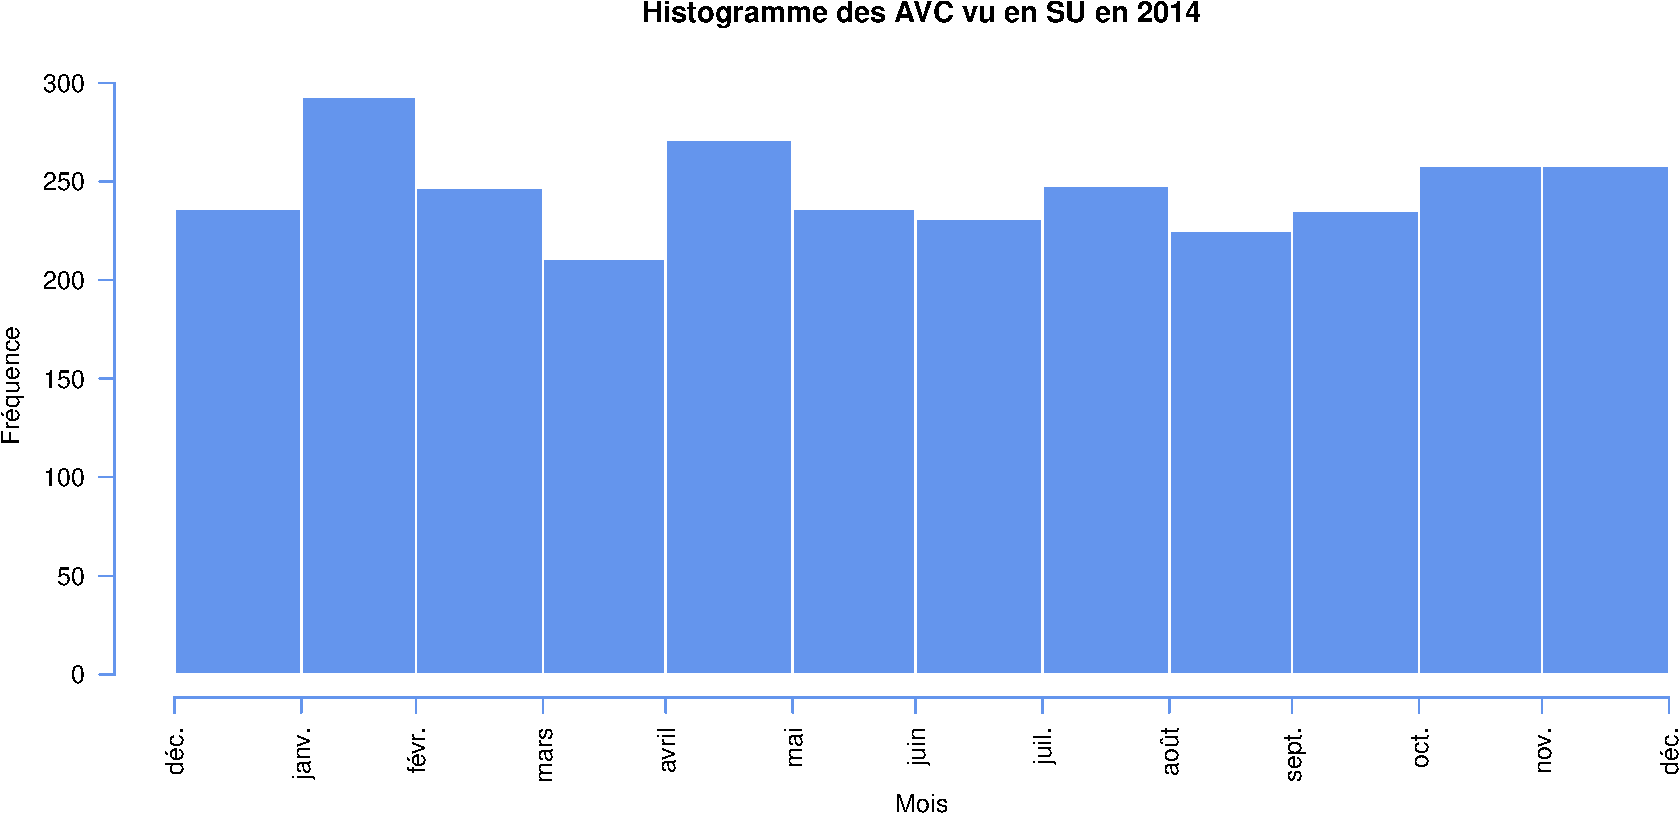
\includegraphics{Figs/hist_avc-1.pdf}

\subsection{Patients}\label{patients-3}

\begin{verbatim}
## c.age
##     [0,5)    [5,10)   [10,15)   [15,20)   [20,25)   [25,30)   [30,35) 
##        10         2         4        10        19        26        26 
##   [35,40)   [40,45)   [45,50)   [50,55)   [55,60)   [60,65)   [65,70) 
##        33        68        97       150       166       235       284 
##   [70,75)   [75,80)   [80,85)   [85,90)   [90,95)  [95,100) [100,105) 
##       295       393       496       408       193        28         4 
## [105,110) [110,115) [115,120) 
##         1         1         0
\end{verbatim}

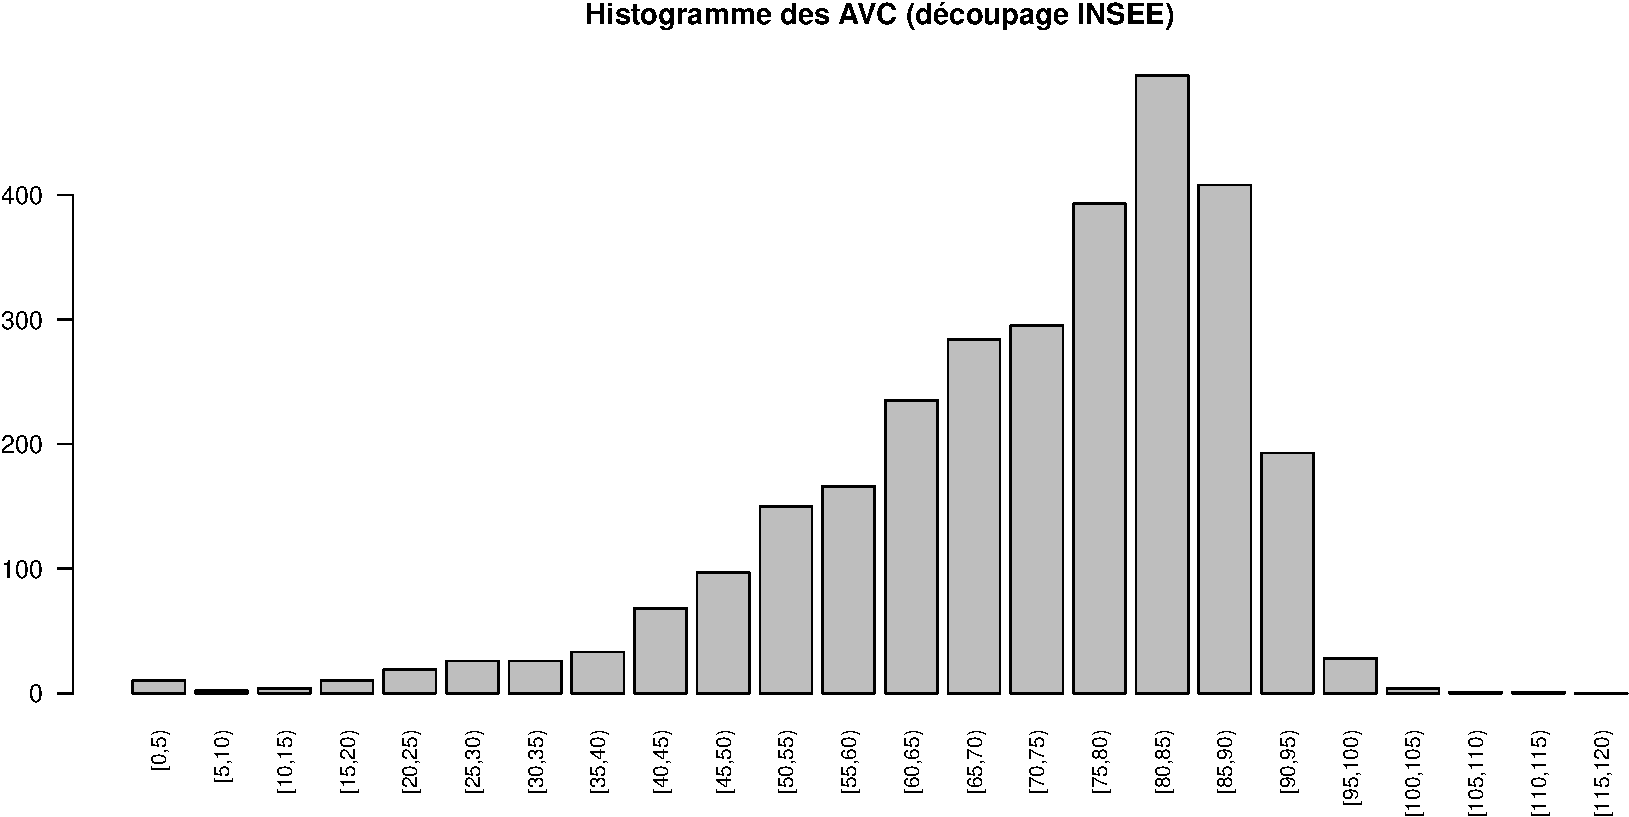
\includegraphics{Figs/Patients-1.pdf}

\begin{verbatim}
## c.age
##    [0,1)    [1,5)   [5,10)  [10,15)  [15,18)  [18,30)  [30,45)  [45,65) 
##        3        7        2        4        4       51      127      648 
##  [65,75)  [75,85) [85,120) 
##      579      889      635
\end{verbatim}

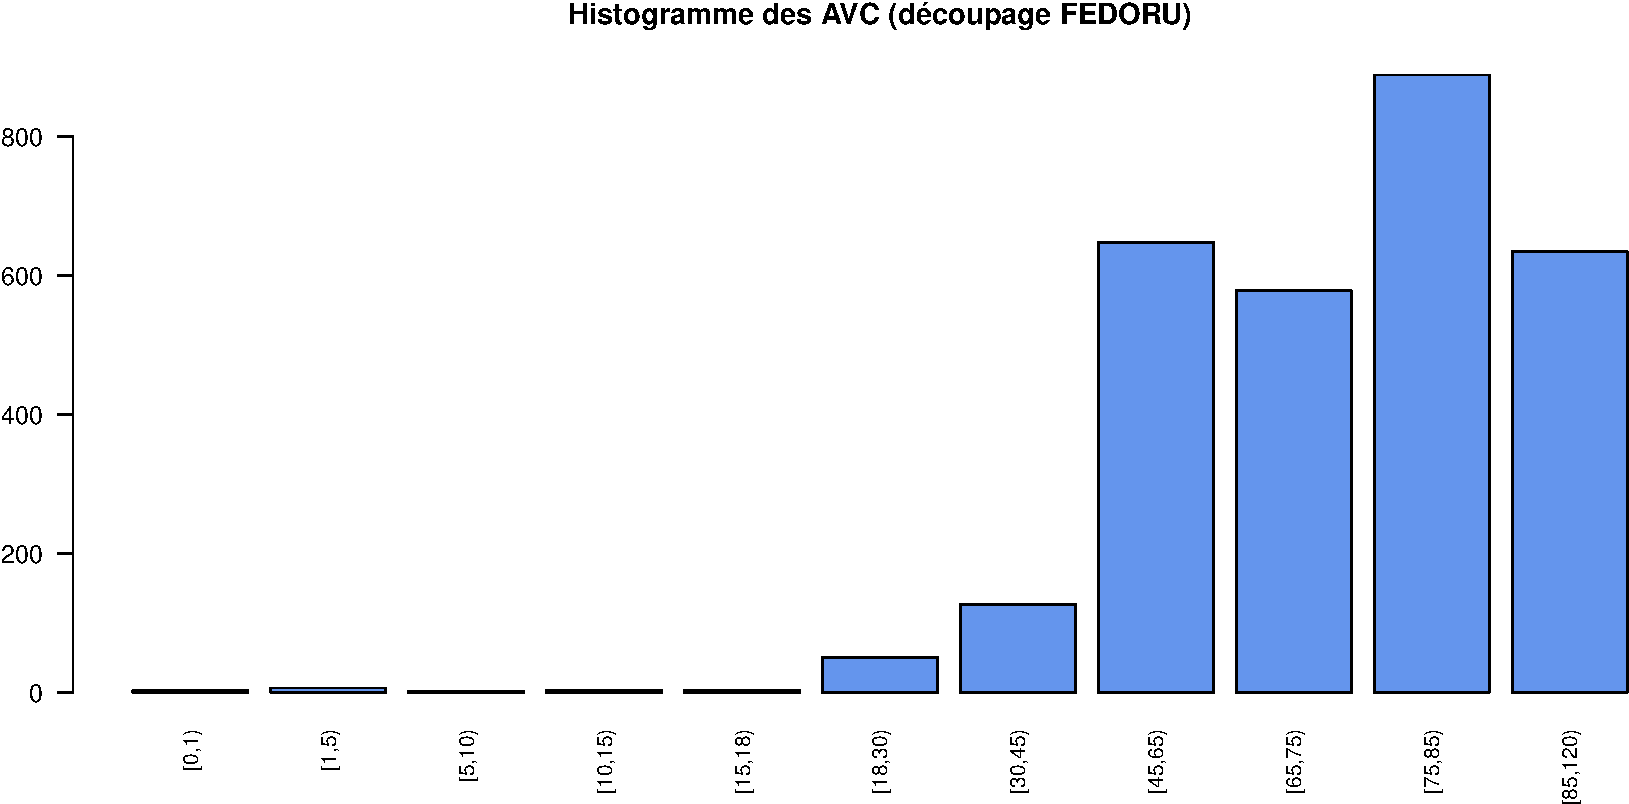
\includegraphics{Figs/Patients-2.pdf}

\begin{itemize}
\itemsep1pt\parskip0pt\parsep0pt
\item
  Sex ratio: 0.95
\item
  Age moyen: 71.44 ans
\item
  Nombre d'AVC par sous classe d'âge (GT1):

  \begin{itemize}
  \itemsep1pt\parskip0pt\parsep0pt
  \item
    85 ans ou moins: 2 404 (81.52 \%)
  \item
    plus de 85 ans: 545 (18.48 \%)
  \end{itemize}
\end{itemize}

\subsection{ARRIVÉE}\label{arrivee-2}

\begin{itemize}
\itemsep1pt\parskip0pt\parsep0pt
\item
  Nombre d'AVC et \% par tranche d'heure GT1 (matinée, début d'après
  midi, fin d'après midi, soirée, nuit profonde)
\end{itemize}

\begin{table}[ht]
\centering
\begin{tabular}{rlllll}
  \hline
 & nuit profonde & matinée & début après-midi & fin après-midi & soirée \\ 
  \hline
Heures & [0,8) & [8,12) & [12,16) & [16,20) & [20,24) \\ 
  Nombre & 272 & 900 & 865 & 619 & 293 \\ 
  \% & 9.22 & 30.52 & 29.33 & 20.99 & 9.94 \\ 
   \hline
\end{tabular}
\caption{Arrivées des AVC} 
\label{avc.arrive}
\end{table}

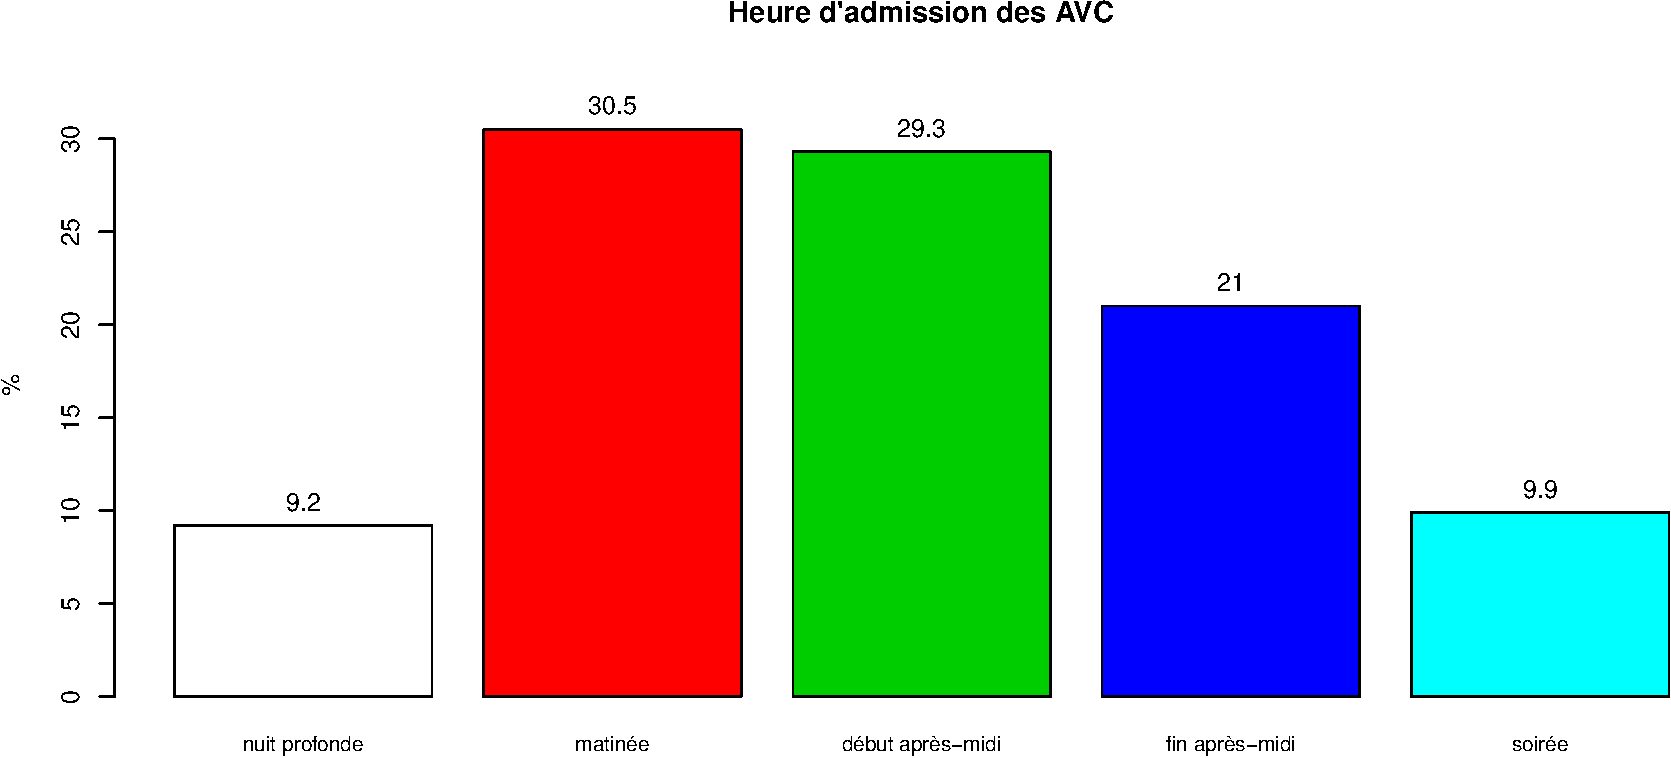
\includegraphics{Figs/avc_periode-1.pdf}

\begin{itemize}
\item
  \% AVC le matin: 30.5 \%.
\item
  \% AVC en début d'après-midi: 29.3 \%.
\item
  \% AVC en fin d'après-midi: 21 \%.
\item
  \% AVC en soirée: 9.9 \%.
\item
  \% AVC le nuit profonde: 9.2 \%.
\item
  Nombre de passages AVC urgences, déclinaison par département,
  établissement, année N

  \begin{table}[ht]
  \centering
  \begin{tabular}{rrr}
    \hline
   & Nombre d'AVC & \% des diagnostics \\ 
    \hline
  3Fr & 63.00 & 0.57 \\ 
    Alk & 30.00 & 0.43 \\ 
    Ane &  &  \\ 
    Col & 741.00 & 1.25 \\ 
    Dia &  &  \\ 
    Dts &  &  \\ 
    Geb & 30.00 & 0.19 \\ 
    Hag & 500.00 & 1.48 \\ 
    Hus & 580.00 & 2.06 \\ 
    Mul & 682.00 & 1.45 \\ 
    Odi &  &  \\ 
    Ros &  &  \\ 
    Sav &  &  \\ 
    Sel & 238.00 & 0.86 \\ 
    Wis & 85.00 & 0.78 \\ 
     \hline
  \end{tabular}
  \caption{Nombre d'AVC par établissement et pourcentage des diagnostics d'AVC parmis l'ensemble des diagnostics principaux évoqués par établissement de santé.} 
  \label{avcParES}
  \end{table}
\item
  \% passages en horaire de PDS

  \begin{longtable}[c]{@{}rlll@{}}
  \toprule
  PDS & S PDS & WE NPD & S\tabularnewline
  \midrule
  \endhead
  Nombre AVC & 403 & 656 & 1890\tabularnewline
  \% AVC & 14 & 22 & 64\tabularnewline
  \bottomrule
  \end{longtable}
\end{itemize}

PDSS = horaires de PDS en semaine, PDSWE = horaires de PDS le WE, NPDS =
hors horaire de PDS.

\begin{itemize}
\itemsep1pt\parskip0pt\parsep0pt
\item
  nombre d'AVC aux horaires de PDS en semaine: 13.67 \%
\item
  nombre d'AVC aux horaires de PDS de week-end:22.24 \%
\item
  nombre d'AVC en dehors des horaires de PDS:64.09 \%
\item
  Nombre de RPU avec diag AVC avec date et heure d'entrées renseignées:
  2 949
\end{itemize}

\subsection{Mode d'arrivée aux
urgences}\label{mode-darrivee-aux-urgences}

\begin{itemize}
\itemsep1pt\parskip0pt\parsep0pt
\item
  Nombre de RPU avec moyens de transport précisé: 2 395
\item
  \% d'arrivées Moyen perso: 21.57\%
\item
  \% d'arrivées SMUR: 1.97\%
\item
  \% d'arrivées VSAV: 17.87\%
\item
  \% d'arrivées ambulance privée: 39.13\% NB : commentaire possible pour
  expliquer que la somme des 4 pourcentages ci dessus ne fait pas 100 \%
\end{itemize}

\subsection{Diagnostic principal}\label{diagnostic-principal-2}

\begin{itemize}
\itemsep1pt\parskip0pt\parsep0pt
\item
  Nombre d'AVC ischémiques et \%: 1 021 (34.62 \%)
\item
  Nombre d'AVC hémorragiques et \%: 442 (14.99 \%)
\item
  Nombre d'AIT et \%: 806 (27.33 \%)
\item
  Nombre de codes ``symptomatiques'' (hémiplégie, aphasie, amaurose,
  etc\ldots{}) et \%: 680 (23.06 \%)
\end{itemize}

NB : se référer à l'annexe 4 pour les regroupements.

\subsection{DURÉE}\label{duree-1}

Voir ligne 333

Voir les routines de RPU\_2014/Analyse/Temps\_passage/passage.R et
notamment \textbf{temps de passage}.

\begin{itemize}
\item
  Nombre de RPU avec une heure de sortie conforme ({]}0-72h{[}: 1 899
\item
  Durée moyenne de passage des Patients PEC pour AVC (en min): 290
\item
  Durée médiane de passage des Patients PEC pour AVC (en min): 255
\item
  Nombre de RPU ac diag AVC dont la durée de passage est inférieure à
  4h: 878
\item
  Durée de passage (HORS UHCD) année N: moyenne \textbf{249.8} minutes,
  et médiane \textbf{228} minutes.
\item
  \% de passages de moins de 4h 0.92
\end{itemize}

\subsection{MODE DE SORTIE}\label{mode-de-sortie-2}

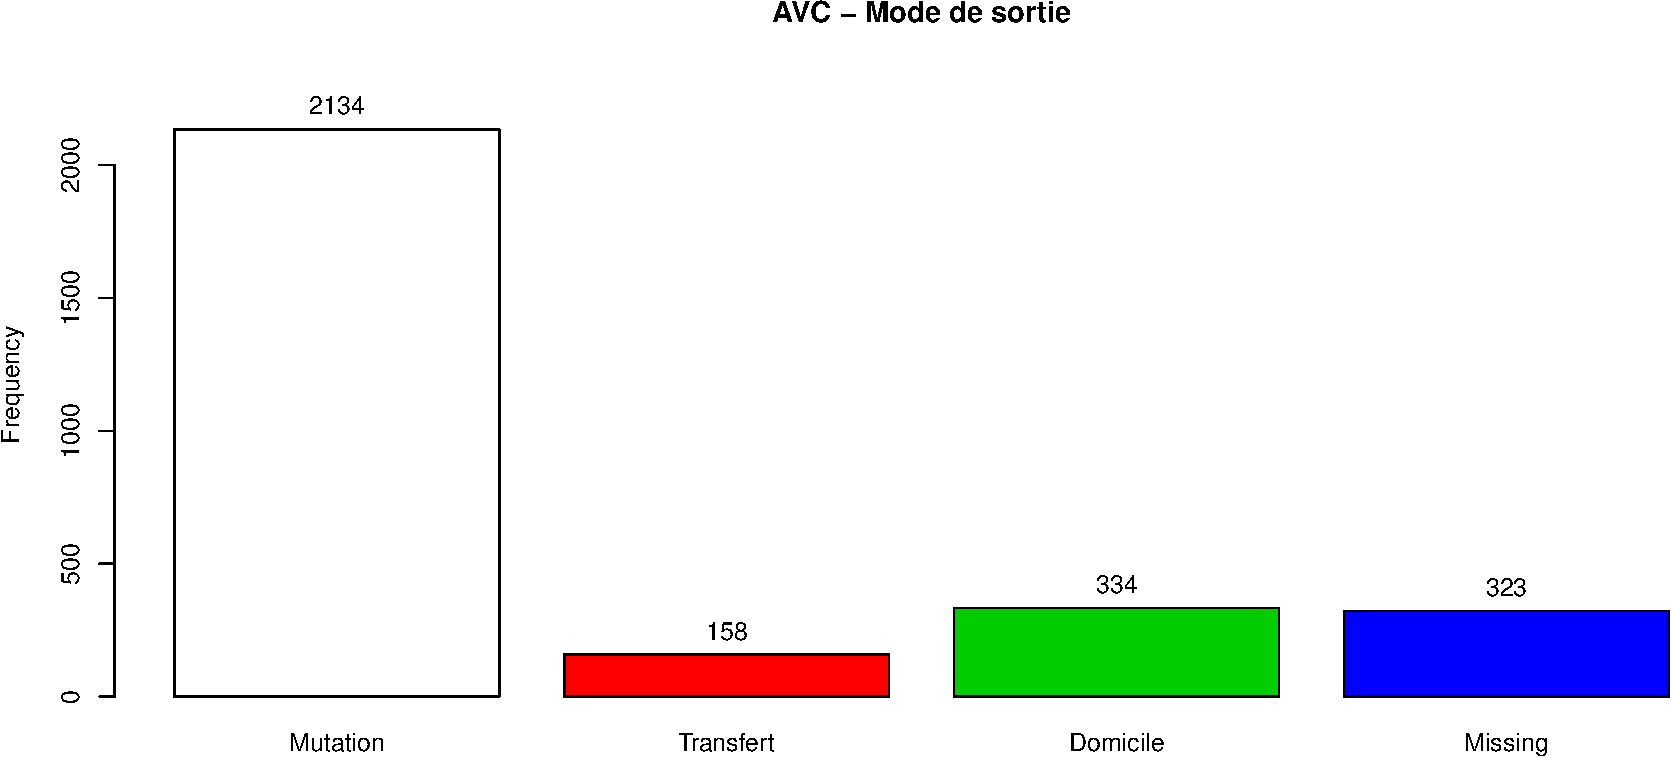
\includegraphics{Figs/avc_mode_sortie-1.pdf}

\begin{itemize}
\itemsep1pt\parskip0pt\parsep0pt
\item
  Nombre de RPU ac diag. AVC avec un mode de sortie renseigné: 2626
\item
  \% d'hospitalisation: 87.3 \% (N = 2292)
\item
  \% de mutation: 81.3 \% (N = 2134)
\item
  \% de transfert: 6 \% (N = 158)
\item
  \% de retour à domicile: 12.7 \% (N = 334)
\end{itemize}

\subsection{Orientation}\label{orientation}

\begin{itemize}
\itemsep1pt\parskip0pt\parsep0pt
\item
  Répartition par orientation en pourcentage, année N
\end{itemize}

\% Table created by stargazer v.5.2 by Marek Hlavac, Harvard University.
E-mail: hlavac at fas.harvard.edu \% Date and time: sam., oct. 31, 2015
- 20:08:14

\begin{table}[!htbp] \centering 
  \caption{Orientation des AVC} 
  \label{orientation} 
\begin{tabular}{@{\extracolsep{5pt}} cccccccccc} 
\\[-1.8ex]\hline 
\hline \\[-1.8ex] 
CHIR & FUGUE & HO & MED & REA & SC & SCAM & SI & UHCD & NA's \\ 
\hline \\[-1.8ex] 
$75$ & $1$ & $1$ & $720$ & $68$ & $46$ & $9$ & $361$ & $919$ & $749$ \\ 
\hline \\[-1.8ex] 
\end{tabular} 
\end{table}

\section{Analyse par type
d'étblissement}\label{analyse-par-type-detblissement}

\subsection{SU de CHU}\label{su-de-chu}

Un seul établissement \textbf{HUS} avec 3 SU:

\begin{itemize}
\itemsep1pt\parskip0pt\parsep0pt
\item
  NHC
\item
  HTP Adultes
\item
  HTP Pédiatrie
\end{itemize}

\textbf{AVERTISSEMENT}: \emph{Les chiffres des HUS sont très
difficilement interprétables en 2014. Du fait d'une anomalie du logiciel
récupérant les RPU avant de les transmettre au concentrateur régional,
le nombreux RPU sont manquants ou incomplet. L'erreur a été corrigée au
mois d'octobre 2014 et seul les deux derniers mois de 2014 sont
fiables.}

\begin{itemize}
\itemsep1pt\parskip0pt\parsep0pt
\item
  Nombre de passages déclarés: 61 793 en 2014.
\item
  Nombre de RPU avec un âge renseigné: 61 793.
\item
  Nombre de RPU avec un code postal renseigné: 61 793.
\item
  Nombre de passages par jour de la semaine:
\end{itemize}

\begin{table}[ht]
\centering
\begin{tabular}{rlll}
  \hline
 & Jour & n & \% \\ 
  \hline
1 & Lun & 9 211 & 14.91 \\ 
  2 & Mar & 8 980 & 14.53 \\ 
  3 & Mer & 8 527 & 13.8 \\ 
  4 & Jeu & 8 667 & 14.03 \\ 
  5 & Ven & 9 170 & 14.84 \\ 
  6 & Sam & 8 806 & 14.25 \\ 
  7 & Dim & 8 432 & 13.65 \\ 
   \hline
\end{tabular}
\caption{Nombre de RPU par jour de semaine} 
\end{table}

\begin{itemize}
\itemsep1pt\parskip0pt\parsep0pt
\item
  Nombre d'âges renseignés: 61 793
\end{itemize}

\begin{table}[ht]
\centering
\begin{tabular}{rlll}
  \hline
 & Tranches d'âge & n & \% \\ 
  \hline
Moins de 1 an & n.inf1an &  2 888 & 9.72 \\ 
  Moins de 15 ans & n.inf15ans & 14 472 & 48.73 \\ 
  75 ans et plus & n.75ans & 12 337 & 41.54 \\ 
   \hline
\end{tabular}
\caption{CHU Alsace 2014 - Nombre de RPU par tranches d'âge} 
\end{table}

\begin{itemize}
\item
  Nombre de passages la nuit: 22 681 (36.7 \%)
\item
  Nombre de passages en horaire de PDS:

  \begin{table}[ht]
  \centering
  \begin{tabular}{rlll}
    \hline
   & Jour & n & \% \\ 
    \hline
  1 & NPDS & 30 243 & 48.94 \\ 
    2 & PDSS & 16 016 & 25.92 \\ 
    3 & PDSWE & 15 534 & 25.14 \\ 
     \hline
  \end{tabular}
  \caption{Passages aux urgences aux horaires de permanence des soins: Passages totaux (NPDS), passages  en semaine (PDSS), passages le week-end (PDSWE)} 
  \end{table}
\item
  Nombre de RPU avec une date-heure d'entrée renseignés: 61 793 (100 \%)
\item
  Nombre de RPU avec une date-heure de sortie renseignés: 48 631 (78.7
  \%)
\item
  Moyen de transport utilisé pour se rendre aux urgences:

  \begin{table}[ht]
  \centering
  \begin{tabular}{rrr}
    \hline
   & n & \% \\ 
    \hline
  Non Renseignés & 53 476,00 & 86,54 \\ 
    Renseignés & 8 317,00 & 13,46 \\ 
    Moyen personnel & 1 214,00 & 14,60 \\ 
    Ambulance & 4 518,00 & 54,32 \\ 
    VSAV & 2 262,00 & 27,20 \\ 
    SMUR & 274,00 & 3,29 \\ 
    Hélicoptère & 2,00 & 0,02 \\ 
    Forces de l'ordre & 47,00 & 0,57 \\ 
     \hline
  \end{tabular}
  \caption{CHU Alsace 2014 - Moyens de transport} 
  \end{table}
\item
  Gravité des RPU évaluée selon la classification CCMU:

  \begin{table}[ht]
  \centering
  \begin{tabular}{rrr}
    \hline
   & n & \% \\ 
    \hline
  Non Renseignés & 28 298,00 & 45,79 \\ 
    Renseignés & 33 495,00 & 54,21 \\ 
    CCMU1 & 8 743,00 & 26,10 \\ 
    CCMU2 & 17 870,00 & 53,35 \\ 
    CCMU3 & 6 178,00 & 18,44 \\ 
    CCMU4 & 503,00 & 1,50 \\ 
    CCMU5 & 201,00 & 0,60 \\ 
    CCMU PSY &  &  \\ 
    CCMU DCD &  &  \\ 
     \hline
  \end{tabular}
  \caption{CHU Alsace 2014 - Gravité des RPU évaluée selon la classification CCMU} 
  \end{table}
\end{itemize}

\subsubsection{Durée de passages}\label{duree-de-passages}

La durée de passage aux urgences est la différence entre l'heure de
sortie et l'heure d'entrée au SU. Dans les calculs qui suivent ne sont
retenus que les RPU qui disposent d'une heure d'entrée et de sortie. Une
durée de passage est considérée comme \textbf{conforme} si elle est
positive et inférieure à 72 heures (FEDORU).

\begin{itemize}
\itemsep1pt\parskip0pt\parsep0pt
\item
  Nombre de durées de passage conformes: 26 416 (42.75 \%)
\item
  Durée moyenne de passage: 254 mn
\item
  Durée médiane de passage: 141 mn
\item
  Durée moyenne de passage en cas de retour à domicile: 827 mn
\item
  Durée médiane de passage en cas de retour à domicile: 664 mn
\item
  Durée moyenne de passage en cas d'hospitalisation: 346 mn
\item
  Durée médiane de passage en cas d'hospitalisation: 312 mn

  \begin{table}[ht]
  \centering
  \begin{tabular}{rrr}
    \hline
   & n & \% \\ 
    \hline
  Nombre de modes de sortie renseignés & 6 278,00 & 23,77 \\ 
    Nombre de modes d'orientation renseignés & 3 170,00 & 12,00 \\ 
    Passages de moins de 4 heures & 17 899,00 & 67,76 \\ 
    Passages $<$ 4h puis hospitalisation & 1 225,00 & 6,84 \\ 
    Passages $<$ 4h puis retour à domicile & 16 674,00 & 93,16 \\ 
    Nombre total de retours à domicile & 2 958,00 & 47,12 \\ 
    Nombre total d'hospitalisations & 3 320,00 & 52,88 \\ 
    nombre total de transferts & 115,00 & 1,83 \\ 
    Nombre total de mutations & 3 205,00 & 51,05 \\ 
    Nombre de déçès & 0,00 & 0,00 \\ 
     \hline
  \end{tabular}
  \caption{CHU Alsace 2014 - Durées de passage selon le devenir du patient} 
  \end{table}
\end{itemize}

\subsection{SU d'ES siège de SAMU, non
CHU}\label{su-des-siege-de-samu-non-chu}

Un seul établissement: CH de Mulhouse avec 2 implantations:

\begin{itemize}
\item
  Emile Muller (Adultes + Pédiatrie traumatique)
\item
  Hasenrain (Pédiatrie médicale)
\item
  Nombre de passages déclarés: 61 793 en 2014.
\item
  Nombre de RPU avec un âge renseigné: 61 793.
\item
  Nombre de RPU avec un code postal renseigné: 61 793.
\item
  Nombre de passages par jour de la semaine:
\end{itemize}

\begin{table}[ht]
\centering
\begin{tabular}{rlll}
  \hline
 & Jour & n & \% \\ 
  \hline
1 & Lun & 9 211 & 14.91 \\ 
  2 & Mar & 8 980 & 14.53 \\ 
  3 & Mer & 8 527 & 13.8 \\ 
  4 & Jeu & 8 667 & 14.03 \\ 
  5 & Ven & 9 170 & 14.84 \\ 
  6 & Sam & 8 806 & 14.25 \\ 
  7 & Dim & 8 432 & 13.65 \\ 
   \hline
\end{tabular}
\caption{Nombre de RPU par jour de semaine} 
\end{table}

\begin{itemize}
\itemsep1pt\parskip0pt\parsep0pt
\item
  Nombre d'âges renseignés: 61 793
\end{itemize}

\begin{table}[ht]
\centering
\begin{tabular}{rlll}
  \hline
 & Tranches d'âge & n & \% \\ 
  \hline
Moins de 1 an & n.inf1an &  2 888 & 9.72 \\ 
  Moins de 15 ans & n.inf15ans & 14 472 & 48.73 \\ 
  75 ans et plus & n.75ans & 12 337 & 41.54 \\ 
   \hline
\end{tabular}
\caption{ES non CHU siège de SAMU 2014 - Nombre de RPU par tranches d'âge} 
\end{table}

\begin{itemize}
\item
  Nombre de passages la nuit: 22 681 (36.7 \%)
\item
  Nombre de passages en horaire de PDS:

  \begin{table}[ht]
  \centering
  \begin{tabular}{rlll}
    \hline
   & Jour & n & \% \\ 
    \hline
  1 & NPDS & 30 243 & 48.94 \\ 
    2 & PDSS & 16 016 & 25.92 \\ 
    3 & PDSWE & 15 534 & 25.14 \\ 
     \hline
  \end{tabular}
  \caption{Passages aux urgences aux horaires de permanence des soins: Passages totaux (NPDS), passages  en semaine (PDSS), passages le week-end (PDSWE)} 
  \end{table}
\item
  Nombre de RPU avec une date-heure d'entrée renseignés: 61 793 (100 \%)
\item
  Nombre de RPU avec une date-heure de sortie renseignés: 48 631 (78.7
  \%)
\item
  Moyen de transport utilisé pour se rendre aux urgences:

  \begin{table}[ht]
  \centering
  \begin{tabular}{rrr}
    \hline
   & n & \% \\ 
    \hline
  Non Renseignés & 53 476,00 & 86,54 \\ 
    Renseignés & 8 317,00 & 13,46 \\ 
    Moyen personnel & 1 214,00 & 14,60 \\ 
    Ambulance & 4 518,00 & 54,32 \\ 
    VSAV & 2 262,00 & 27,20 \\ 
    SMUR & 274,00 & 3,29 \\ 
    Hélicoptère & 2,00 & 0,02 \\ 
    Forces de l'ordre & 47,00 & 0,57 \\ 
     \hline
  \end{tabular}
  \caption{ES non CHU siège de SAMU 2014 - Moyens de transport} 
  \end{table}
\item
  Gravité des RPU évaluée selon la classification CCMU:

  \begin{table}[ht]
  \centering
  \begin{tabular}{rrr}
    \hline
   & n & \% \\ 
    \hline
  Non Renseignés & 28 298,00 & 45,79 \\ 
    Renseignés & 33 495,00 & 54,21 \\ 
    CCMU1 & 8 743,00 & 26,10 \\ 
    CCMU2 & 17 870,00 & 53,35 \\ 
    CCMU3 & 6 178,00 & 18,44 \\ 
    CCMU4 & 503,00 & 1,50 \\ 
    CCMU5 & 201,00 & 0,60 \\ 
    CCMU PSY &  &  \\ 
    CCMU DCD &  &  \\ 
     \hline
  \end{tabular}
  \caption{ES non CHU siège de SAMU 2014 - Gravité des RPU évaluée selon la classification CCMU} 
  \end{table}
\end{itemize}

\subsubsection{Durée de passages}\label{duree-de-passages-1}

La durée de passage aux urgences est la différence entre l'heure de
sortie et l'heure d'entrée au SU. Dans les calculs qui suivent ne sont
retenus que les RPU qui disposent d'une heure d'entrée et de sortie. Une
durée de passage est considérée comme \textbf{conforme} si elle est
positive et inférieure à 72 heures (FEDORU).

\begin{itemize}
\itemsep1pt\parskip0pt\parsep0pt
\item
  Nombre de durées de passage conformes: 26 416 (42.75 \%)
\item
  Durée moyenne de passage: 254 mn
\item
  Durée médiane de passage: 141 mn
\item
  Durée moyenne de passage en cas de retour à domicile: 827 mn
\item
  Durée médiane de passage en cas de retour à domicile: 664 mn
\item
  Durée moyenne de passage en cas d'hospitalisation: 346 mn
\item
  Durée médiane de passage en cas d'hospitalisation: 312 mn

  \begin{table}[ht]
  \centering
  \begin{tabular}{rrr}
    \hline
   & n & \% \\ 
    \hline
  Nombre de modes de sortie renseignés & 6 278,00 & 23,77 \\ 
    Nombre de modes d'orientation renseignés & 3 170,00 & 12,00 \\ 
    Passages de moins de 4 heures & 17 899,00 & 67,76 \\ 
    Passages $<$ 4h puis hospitalisation & 1 225,00 & 6,84 \\ 
    Passages $<$ 4h puis retour à domicile & 16 674,00 & 93,16 \\ 
    Nombre total de retours à domicile & 2 958,00 & 47,12 \\ 
    Nombre total d'hospitalisations & 3 320,00 & 52,88 \\ 
    nombre total de transferts & 115,00 & 1,83 \\ 
    Nombre total de mutations & 3 205,00 & 51,05 \\ 
    Nombre de déçès & 0,00 & 0,00 \\ 
     \hline
  \end{tabular}
  \caption{ES non CHU siège de SAMU 2014 - Durées de passage selon le devenir du patient} 
  \end{table}
\end{itemize}

\subsection{SU avec SMUR non siège de
SAMU}\label{su-avec-smur-non-siege-de-samu}

Les SU non sièges de SAMU, avec SMUR représentent cinq établissements:

\begin{itemize}
\item
  CH Wissembourg
\item
  CH haguenau
\item
  CH Saverne
\item
  CH Sélestat
\item
  CH Colmar
\item
  Nombre de passages déclarés: 177 747 en 2014.
\item
  Nombre de RPU avec un âge renseigné: 177 747.
\item
  Nombre de RPU avec un code postal renseigné: 177 747.
\item
  Nombre de passages par jour de la semaine:
\end{itemize}

\begin{table}[ht]
\centering
\begin{tabular}{rlll}
  \hline
 & Jour & n & \% \\ 
  \hline
1 & Lun & 27 415 & 15.42 \\ 
  2 & Mar & 24 007 & 13.51 \\ 
  3 & Mer & 24 628 & 13.86 \\ 
  4 & Jeu & 24 099 & 13.56 \\ 
  5 & Ven & 24 688 & 13.89 \\ 
  6 & Sam & 25 896 & 14.57 \\ 
  7 & Dim & 27 014 & 15.2 \\ 
   \hline
\end{tabular}
\caption{Nombre de RPU par jour de semaine} 
\end{table}

\begin{itemize}
\itemsep1pt\parskip0pt\parsep0pt
\item
  Nombre d'âges renseignés: 177 747
\end{itemize}

\begin{table}[ht]
\centering
\begin{tabular}{rlll}
  \hline
 & Tranches d'âge & n & \% \\ 
  \hline
Moins de 1 an & n.inf1an &  7 110 & 8.74 \\ 
  Moins de 15 ans & n.inf15ans & 48 795 & 59.98 \\ 
  75 ans et plus & n.75ans & 25 444 & 31.28 \\ 
   \hline
\end{tabular}
\caption{ES non sièges de SAMU, avec SMUR 2014 - Nombre de RPU par tranches d'âge} 
\end{table}

\begin{itemize}
\item
  Nombre de passages la nuit: 46 677 (26.26 \%)
\item
  Nombre de passages en horaire de PDS:

  \begin{table}[ht]
  \centering
  \begin{tabular}{rlll}
    \hline
   & Jour & n & \% \\ 
    \hline
  1 & NPDS & 98 847 & 55.61 \\ 
    2 & PDSS & 32 166 & 18.1 \\ 
    3 & PDSWE & 46 734 & 26.29 \\ 
     \hline
  \end{tabular}
  \caption{Passages aux urgences aux horaires de permanence des soins: Passages totaux (NPDS), passages  en semaine (PDSS), passages le week-end (PDSWE)} 
  \end{table}
\item
  Nombre de RPU avec une date-heure d'entrée renseignés: 177 747 (100
  \%)
\item
  Nombre de RPU avec une date-heure de sortie renseignés: 168 547 (94.82
  \%)
\item
  Moyen de transport utilisé pour se rendre aux urgences:

  \begin{table}[ht]
  \centering
  \begin{tabular}{rrr}
    \hline
   & n & \% \\ 
    \hline
  Non Renseignés & 41 213,00 & 23,19 \\ 
    Renseignés & 136 534,00 & 76,81 \\ 
    Moyen personnel & 97 489,00 & 71,40 \\ 
    Ambulance & 21 771,00 & 15,95 \\ 
    VSAV & 14 816,00 & 10,85 \\ 
    SMUR & 1 603,00 & 1,17 \\ 
    Hélicoptère & 95,00 & 0,07 \\ 
    Forces de l'ordre & 760,00 & 0,56 \\ 
     \hline
  \end{tabular}
  \caption{ES non sièges de SAMU, avec SMUR 2014 - Moyens de transport} 
  \end{table}
\item
  Gravité des RPU évaluée selon la classification CCMU:

  \begin{table}[ht]
  \centering
  \begin{tabular}{rrr}
    \hline
   & n & \% \\ 
    \hline
  Non Renseignés & 21 649,00 & 12,18 \\ 
    Renseignés & 156 098,00 & 87,82 \\ 
    CCMU1 & 27 108,00 & 17,37 \\ 
    CCMU2 & 101 455,00 & 64,99 \\ 
    CCMU3 & 24 309,00 & 15,57 \\ 
    CCMU4 & 1 547,00 & 0,99 \\ 
    CCMU5 & 385,00 & 0,25 \\ 
    CCMU PSY & 1 273,00 & 0,82 \\ 
    CCMU DCD & 21,00 & 0,01 \\ 
     \hline
  \end{tabular}
  \caption{ES non sièges de SAMU, avec SMUR 2014 - Gravité des RPU évaluée selon la classification CCMU} 
  \end{table}
\end{itemize}

\subsubsection{Durée de passages}\label{duree-de-passages-2}

La durée de passage aux urgences est la différence entre l'heure de
sortie et l'heure d'entrée au SU. Dans les calculs qui suivent ne sont
retenus que les RPU qui disposent d'une heure d'entrée et de sortie. Une
durée de passage est considérée comme \textbf{conforme} si elle est
positive et inférieure à 72 heures (FEDORU).

\begin{itemize}
\itemsep1pt\parskip0pt\parsep0pt
\item
  Nombre de durées de passage conformes: 158 099 (88.95 \%)
\item
  Durée moyenne de passage: 164 mn
\item
  Durée médiane de passage: 120 mn
\item
  Durée moyenne de passage en cas de retour à domicile: 144 mn
\item
  Durée médiane de passage en cas de retour à domicile: 107 mn
\item
  Durée moyenne de passage en cas d'hospitalisation: 245 mn
\item
  Durée médiane de passage en cas d'hospitalisation: 206 mn

  \begin{table}[ht]
  \centering
  \begin{tabular}{rrr}
    \hline
   & n & \% \\ 
    \hline
  Nombre de modes de sortie renseignés & 156 215,00 & 98,81 \\ 
    Nombre de modes d'orientation renseignés & 30 884,00 & 19,53 \\ 
    Passages de moins de 4 heures & 126 600,00 & 80,08 \\ 
    Passages $<$ 4h puis hospitalisation & 18 044,00 & 14,25 \\ 
    Passages $<$ 4h puis retour à domicile & 108 555,00 & 85,75 \\ 
    Nombre total de retours à domicile & 125 505,00 & 80,34 \\ 
    Nombre total d'hospitalisations & 30 709,00 & 19,66 \\ 
    nombre total de transferts & 2 840,00 & 1,82 \\ 
    Nombre total de mutations & 27 869,00 & 17,84 \\ 
    Nombre de déçès & 1,00 & 0,00 \\ 
     \hline
  \end{tabular}
  \caption{ES non sièges de SAMU, avec SMUR 2014 - Durées de passage selon le devenir du patient} 
  \end{table}
\end{itemize}

\subsection{SU non SMUR, non SAMU, non
CHU}\label{su-non-smur-non-samu-non-chu}

ES avec SU isolé (pas de SMUR associé), 8 établissements: clinique Ste
Anne (GHSV), clinique Ste Odile (RHENA), Diaconat Strasbourg (RHENA), CH
de Guebwiller, CH de Thann (pas de RPU), CH d'Altkirch, Clinique des 3
frontières (GHMSA), Diaconat-Roosvelt, Siaconat-Fonderie.

\begin{itemize}
\itemsep1pt\parskip0pt\parsep0pt
\item
  Nombre de passages déclarés: 117 722 en 2014.
\item
  Nombre de RPU avec un âge renseigné: 117 718.
\item
  Nombre de RPU avec un code postal renseigné: 117 722.
\item
  Nombre de passages par jour de la semaine:
\end{itemize}

\begin{table}[ht]
\centering
\begin{tabular}{rlll}
  \hline
 & Jour & n & \% \\ 
  \hline
1 & Lun & 18 645 & 15.84 \\ 
  2 & Mar & 15 880 & 13.49 \\ 
  3 & Mer & 16 232 & 13.79 \\ 
  4 & Jeu & 16 002 & 13.59 \\ 
  5 & Ven & 16 456 & 13.98 \\ 
  6 & Sam & 17 567 & 14.92 \\ 
  7 & Dim & 16 940 & 14.39 \\ 
   \hline
\end{tabular}
\caption{Nombre de RPU par jour de semaine} 
\end{table}

\begin{itemize}
\itemsep1pt\parskip0pt\parsep0pt
\item
  Nombre d'âges renseignés: 117 718
\end{itemize}

\begin{table}[ht]
\centering
\begin{tabular}{rlll}
  \hline
 & Tranches d'âge & n & \% \\ 
  \hline
Moins de 1 an & n.inf1an &    663 & 1.96 \\ 
  Moins de 15 ans & n.inf15ans & 21 131 & 62.51 \\ 
  75 ans et plus & n.75ans & 12 010 & 35.53 \\ 
   \hline
\end{tabular}
\caption{ES avec SU non SMUR2014 - Nombre de RPU par tranches d'âge} 
\end{table}

\begin{itemize}
\item
  Nombre de passages la nuit: 27 711 (23.54 \%)
\item
  Nombre de passages en horaire de PDS:

  \begin{table}[ht]
  \centering
  \begin{tabular}{rlll}
    \hline
   & Jour & n & \% \\ 
    \hline
  1 & NPDS & 68 659 & 58.32 \\ 
    2 & PDSS & 19 254 & 16.36 \\ 
    3 & PDSWE & 29 809 & 25.32 \\ 
     \hline
  \end{tabular}
  \caption{Passages aux urgences aux horaires de permanence des soins: Passages totaux (NPDS), passages  en semaine (PDSS), passages le week-end (PDSWE)} 
  \end{table}
\item
  Nombre de RPU avec une date-heure d'entrée renseignés: 117 722 (100
  \%)
\item
  Nombre de RPU avec une date-heure de sortie renseignés: 108 873 (92.48
  \%)
\item
  Moyen de transport utilisé pour se rendre aux urgences:

  \begin{table}[ht]
  \centering
  \begin{tabular}{rrr}
    \hline
   & n & \% \\ 
    \hline
  Non Renseignés & 28 900,00 & 24,55 \\ 
    Renseignés & 88 822,00 & 75,45 \\ 
    Moyen personnel & 74 095,00 & 83,42 \\ 
    Ambulance & 8 035,00 & 9,05 \\ 
    VSAV & 5 825,00 & 6,56 \\ 
    SMUR & 602,00 & 0,68 \\ 
    Hélicoptère & 1,00 & 0,00 \\ 
    Forces de l'ordre & 264,00 & 0,30 \\ 
     \hline
  \end{tabular}
  \caption{ES avec SU non SMUR2014 - Moyens de transport} 
  \end{table}
\item
  Gravité des RPU évaluée selon la classification CCMU:

  \begin{table}[ht]
  \centering
  \begin{tabular}{rrr}
    \hline
   & n & \% \\ 
    \hline
  Non Renseignés & 12 916,00 & 10,97 \\ 
    Renseignés & 104 806,00 & 89,03 \\ 
    CCMU1 & 8 482,00 & 8,09 \\ 
    CCMU2 & 85 521,00 & 81,60 \\ 
    CCMU3 & 10 593,00 & 10,11 \\ 
    CCMU4 & 147,00 & 0,14 \\ 
    CCMU5 & 24,00 & 0,02 \\ 
    CCMU PSY & 34,00 & 0,03 \\ 
    CCMU DCD & 5,00 & 0,00 \\ 
     \hline
  \end{tabular}
  \caption{ES avec SU non SMUR2014 - Gravité des RPU évaluée selon la classification CCMU} 
  \end{table}
\end{itemize}

\subsubsection{Durée de passages}\label{duree-de-passages-3}

La durée de passage aux urgences est la différence entre l'heure de
sortie et l'heure d'entrée au SU. Dans les calculs qui suivent ne sont
retenus que les RPU qui disposent d'une heure d'entrée et de sortie. Une
durée de passage est considérée comme \textbf{conforme} si elle est
positive et inférieure à 72 heures (FEDORU).

\begin{itemize}
\itemsep1pt\parskip0pt\parsep0pt
\item
  Nombre de durées de passage conformes: 106 689 (90.63 \%)
\item
  Durée moyenne de passage: 120 mn
\item
  Durée médiane de passage: 87 mn
\item
  Durée moyenne de passage en cas de retour à domicile: 114 mn
\item
  Durée médiane de passage en cas de retour à domicile: 84 mn
\item
  Durée moyenne de passage en cas d'hospitalisation: 174 mn
\item
  Durée médiane de passage en cas d'hospitalisation: 135 mn

  \begin{table}[ht]
  \centering
  \begin{tabular}{rrr}
    \hline
   & n & \% \\ 
    \hline
  Nombre de modes de sortie renseignés & 95 563,00 & 89,57 \\ 
    Nombre de modes d'orientation renseignés & 6 740,00 & 6,32 \\ 
    Passages de moins de 4 heures & 96 529,00 & 90,48 \\ 
    Passages $<$ 4h puis hospitalisation & 7 050,00 & 7,30 \\ 
    Passages $<$ 4h puis retour à domicile & 89 478,00 & 92,70 \\ 
    Nombre total de retours à domicile & 86 531,00 & 90,55 \\ 
    Nombre total d'hospitalisations & 9 031,00 & 9,45 \\ 
    nombre total de transferts & 2 575,00 & 2,69 \\ 
    Nombre total de mutations & 6 456,00 & 6,76 \\ 
    Nombre de déçès & 1,00 & 0,00 \\ 
     \hline
  \end{tabular}
  \caption{ES avec SU non SMUR2014 - Durées de passage selon le devenir du patient} 
  \end{table}
\end{itemize}

\section{Test de la routine et tableau
compact}\label{test-de-la-routine-et-tableau-compact}

En fonction du type de structures d'urgences disponibles, on peut
distingur quatre catégories d'établissements:

\begin{itemize}
\itemsep1pt\parskip0pt\parsep0pt
\item
  Catégorie 1: Les SU de CHU (SAMU, SMUR, Urgences adultes et enfants).
\item
  Catégorie 2: Les SU non CHU, sièges de SAMU.
\item
  Catégorie 3: Les SU non CHU, non SAMU, sièges de SMUR.
\item
  Catégorie 4: Les SU simples.
\end{itemize}

\begin{table}[ht]
\centering
\begin{tabular}{rrrrr}
  \hline
 & Catégorie 1 & Catégorie 2 & Catégorie 3 & Catégorie 4 \\ 
  \hline
n.passages & 61793.00 & 59471.00 & 177747.00 & 117722.00 \\ 
  n.age.ren & 61793.00 & 59471.00 & 177747.00 & 117718.00 \\ 
  n.inf1an & 2888.00 & 4715.00 & 7110.00 & 663.00 \\ 
  n.inf15ans & 14472.00 & 19015.00 & 48795.00 & 21131.00 \\ 
  n.75ans & 12337.00 & 7480.00 & 25444.00 & 12010.00 \\ 
  n.cp.rens & 61793.00 & 59471.00 & 177747.00 & 117722.00 \\ 
  n.etrangers & 2505.00 & 1519.00 & 11071.00 & 3372.00 \\ 
  n.lun & 9211.00 & 8868.00 & 27415.00 & 18645.00 \\ 
  n.mar & 8980.00 & 7885.00 & 24007.00 & 15880.00 \\ 
  n.mer & 8527.00 & 8130.00 & 24628.00 & 16232.00 \\ 
  n.jeu & 8667.00 & 7931.00 & 24099.00 & 16002.00 \\ 
  n.ven & 9170.00 & 8270.00 & 24688.00 & 16456.00 \\ 
  n.sam & 8806.00 & 8854.00 & 25896.00 & 17567.00 \\ 
  n.dim & 8432.00 & 9533.00 & 27014.00 & 16940.00 \\ 
  n.nuit & 22681.00 & 18349.00 & 46677.00 & 27711.00 \\ 
  n.pds & 31550.00 & 28941.00 & 78900.00 & 49063.00 \\ 
  n.h.rens & 61793.00 & 59471.00 & 177747.00 & 117722.00 \\ 
  n.trans.rens & 8317.00 & 55635.00 & 136534.00 & 88822.00 \\ 
  n.fo & 47.00 & 478.00 & 760.00 & 264.00 \\ 
  n.heli & 2.00 & 122.00 & 95.00 & 1.00 \\ 
  n.perso & 1214.00 & 35973.00 & 97489.00 & 74095.00 \\ 
  n.smur & 274.00 & 223.00 & 1603.00 & 602.00 \\ 
  n.vsav & 2262.00 & 7051.00 & 14816.00 & 5825.00 \\ 
  n.ambu & 4518.00 & 11788.00 & 21771.00 & 8035.00 \\ 
  n.ccmu.rens & 33495.00 & 45428.00 & 156098.00 & 104806.00 \\ 
  n.ccmu1 & 8743.00 & 7349.00 & 27108.00 & 8482.00 \\ 
  n.ccmu2 & 17870.00 & 30451.00 & 101455.00 & 85521.00 \\ 
  n.ccmu3 & 6178.00 & 6094.00 & 24309.00 & 10593.00 \\ 
  n.ccmu4 & 503.00 & 1235.00 & 1547.00 & 147.00 \\ 
  n.ccmu5 & 201.00 & 299.00 & 385.00 & 24.00 \\ 
  n.ccmuP &  &  & 1273.00 & 34.00 \\ 
  n.ccmuD &  &  & 21.00 & 5.00 \\ 
  n.ccmu45 & 704.00 & 1534.00 & 1932.00 & 171.00 \\ 
  n.sorties.conf & 26416.00 & 47518.00 & 158099.00 & 106689.00 \\ 
  mean.passage & 254.03 & 184.40 & 163.53 & 119.78 \\ 
  median.passage & 141.00 & 151.00 & 120.00 & 87.00 \\ 
  n.passage4 & 17899.00 & 34593.00 & 126600.00 & 96529.00 \\ 
  n.hosp.passage4 & 1225.00 & 4159.00 & 18044.00 & 7050.00 \\ 
  n.dom.passage4 & 16674.00 & 30434.00 & 108555.00 & 89478.00 \\ 
  n.dom & 2958.00 & 35746.00 & 125505.00 & 86531.00 \\ 
  n.hosp & 3320.00 & 7543.00 & 30709.00 & 9031.00 \\ 
  n.transfert & 115.00 & 135.00 & 2840.00 & 2575.00 \\ 
  n.deces & 0.00 & 0.00 & 1.00 & 1.00 \\ 
  n.mode.sortie & 26456.00 & 45214.00 & 167532.00 & 99676.00 \\ 
  n.mutation2 & 23219.00 & 8347.00 & 37564.00 & 7869.00 \\ 
   \hline
\end{tabular}
\caption{Chiffres clés des SU d'Alsace en 2014 - Synthèse des données en fonction de la catégorie d'établissement.} 
\end{table}

En pourcentages:

\begin{table}[ht]
\centering
\begin{tabular}{rrrrr}
  \hline
 & Catégorie 1 & Catégorie 2 & Catégorie 3 & Catégorie 4 \\ 
  \hline
p.age.ren & 100.00 & 100.00 & 100.00 & 100.00 \\ 
  p.inf1an & 4.67 & 7.93 & 4.00 & 0.56 \\ 
  p.inf15ans & 23.42 & 31.97 & 27.45 & 17.95 \\ 
  p.75ans & 19.97 & 12.58 & 14.31 & 10.20 \\ 
  p.cp.rens & 100.00 & 100.00 & 100.00 & 100.00 \\ 
  p.etrangers &  &  &  &  \\ 
  p.lun & 921100.00 & 886800.00 & 2741500.00 & 1864500.00 \\ 
  p.mar & 898000.00 & 788500.00 & 2400700.00 & 1588000.00 \\ 
  p.mer & 852700.00 & 813000.00 & 2462800.00 & 1623200.00 \\ 
  p.jeu & 866700.00 & 793100.00 & 2409900.00 & 1600200.00 \\ 
  p.ven & 917000.00 & 827000.00 & 2468800.00 & 1645600.00 \\ 
  p.sam & 880600.00 & 885400.00 & 2589600.00 & 1756700.00 \\ 
  p.dim & 843200.00 & 953300.00 & 2701400.00 & 1694000.00 \\ 
  p.nuit & 2268100.00 & 1834900.00 & 4667700.00 & 2771100.00 \\ 
  p.pds & 3155000.00 & 2894100.00 & 7890000.00 & 4906300.00 \\ 
  p.h.rens & 100.00 & 100.00 & 100.00 & 100.00 \\ 
  p.trans.rens & 13.46 & 93.55 & 76.81 & 75.45 \\ 
  p.fo & 0.57 & 0.86 & 0.56 & 0.30 \\ 
  p.heli & 0.02 & 0.22 & 0.07 & 0.00 \\ 
  p.perso & 14.60 & 64.66 & 71.40 & 83.42 \\ 
  p.smur & 3.29 & 0.40 & 1.17 & 0.68 \\ 
  p.vsav & 27.20 & 12.67 & 10.85 & 6.56 \\ 
  p.ambu & 54.32 & 21.19 & 15.95 & 9.05 \\ 
  p.ccmu.rens & 54.21 & 76.39 & 87.82 & 89.03 \\ 
  p.ccmu1 & 26.10 & 16.18 & 17.37 & 8.09 \\ 
  p.ccmu2 & 53.35 & 67.03 & 64.99 & 81.60 \\ 
  p.ccmu3 & 18.44 & 13.41 & 15.57 & 10.11 \\ 
  p.ccmu4 & 1.50 & 2.72 & 0.99 & 0.14 \\ 
  p.ccmu5 & 0.60 & 0.66 & 0.25 & 0.02 \\ 
  p.ccmuP &  &  & 0.82 & 0.03 \\ 
  p.ccmuD &  &  & 0.01 & 0.00 \\ 
  p.ccmu45 & 2.10 & 3.38 & 1.24 & 0.16 \\ 
  p.sorties.conf &  &  &  &  \\ 
  p.passage4 & 67.76 & 72.80 & 80.08 & 90.48 \\ 
  p.hosp.passage4 & 6.84 & 12.02 & 14.25 & 7.30 \\ 
  p.dom.passage4 & 93.16 & 87.98 & 85.75 & 92.70 \\ 
  p.dom & 47.12 & 82.58 & 80.34 & 90.55 \\ 
  p.hosp & 52.88 & 17.42 & 19.66 & 9.45 \\ 
  p.transfert & 1.83 & 0.31 & 1.82 & 2.69 \\ 
  p.deces & 0.00 & 0.00 & 0.00 & 0.00 \\ 
  p.mode.sortie & 42.81 & 76.03 & 94.25 & 84.67 \\ 
  p.mutation2 & 87.76 & 18.46 & 22.42 & 7.89 \\ 
   \hline
\end{tabular}
\caption{Chiffres clés des SU d'Alsace en 2014 - Synthèse des données, exprimées en pourcentage, en fonction de la catégorie d'établissement.} 
\end{table}

\section{Comparaison à hôpitaux
constants}\label{comparaison-a-hopitaux-constants}

Introduit dans le rapoort 2014: pour évaluer le taux de progression
2013-2014, on compare uniquement les hôpitaux de 2014 qui transmettaient
déjà des données en 2013:

\begin{verbatim}
## [1] 0.17
\end{verbatim}

\begin{verbatim}
## [1] 115051
\end{verbatim}

\begin{verbatim}
## [1] 56061
\end{verbatim}

\section{ANNEXES}\label{annexes}

\subsection{ANNEXE 1 : Définitions}\label{annexe-1-definitions}

\subsection{Définitions et méthodes}\label{definitions-et-methodes}

\subsubsection{Durée de passage}\label{duree-de-passage-1}

Délais en minutes ou en heures entre la date de sortie et la date
d'entrée. Les passages dont la durée n'est pas calculable, négative,
nulle ou supérieure à 72 heures, ne sont pas prises en compte.

\subsubsection{Journée et nuit}\label{journee-et-nuit}

\begin{itemize}
\itemsep1pt\parskip0pt\parsep0pt
\item
  Journée = {[}08h00 - 19h59{]}
\item
  Nuit = {[}20h00 - 07h59{]}
\item
  Soirée = {[}20h00 - 23h59{]}
\item
  Nuit profonde = {[}00h00 - 07h59{]}
\end{itemize}

\subsubsection{Semaine et week-end}\label{semaine-et-week-end}

\begin{itemize}
\itemsep1pt\parskip0pt\parsep0pt
\item
  Semaine = {[}Lundi 00h00 - Vendredi 23h59{]}
\item
  Week-end = {[}Samedi 00h00 - Dimanche 23h59{]}
\end{itemize}

\subsubsection{Permanence des soins
(PDS)}\label{permanence-des-soins-pds}

\begin{itemize}
\itemsep1pt\parskip0pt\parsep0pt
\item
  Tous les jours de la semaine en horaire de nuit
\item
  le samedi de 12h à 19h59
\item
  le dimanche, les jours fériés et les ponts de 08h00 à 19h59
\end{itemize}

\subsubsection{Sex-ratio}\label{sex-ratio}

\begin{itemize}
\itemsep1pt\parskip0pt\parsep0pt
\item
  Sex-ratio: c'est le nombre d'hommes divisé par le nombre de femmes
\item
  Taux de masculinité: c'est le nombre d'hommes divisé par le nombre de
  personnes (hommes + femmes)
\end{itemize}

\subsubsection{Âge}\label{age}

Âge = date d'entrée - date de naissance. Les ages négatifs ou supérieurs
à 120 ans ne sont pas pris en compte.

\subsubsection{Pédiatrie}\label{pediatrie}

Tous les patients dont l'âge est inférieur à 18 ans.

\subsubsection{Gériatrie}\label{geriatrie}

Tous les patients dont l'âge est égal ou supérieur à 75 ans.

\subsection{ANNEXE 2 : Diagramme de complétude des
RPU}\label{annexe-2-diagramme-de-completude-des-rpu}

\subsection{ANNEXE 3 : Méthodologie}\label{annexe-3-methodologie}

\subsubsection{Calcul du TARRU}\label{calcul-du-tarru}

taux de recours (de la région ou département) : nombre de passages dans
les services d'urgences (de la région ou département) de patients
résidant dans une zone donnée (code postal ou commune) divisé par la
population estimée de cette zone sur la période donnée.

\section{Information de session}\label{information-de-session}

\begin{verbatim}
R version 3.2.2 (2015-08-14)
Platform: x86_64-pc-linux-gnu (64-bit)
Running under: Ubuntu 14.04.3 LTS

locale:
 [1] LC_CTYPE=fr_FR.UTF-8       LC_NUMERIC=C              
 [3] LC_TIME=fr_FR.UTF-8        LC_COLLATE=fr_FR.UTF-8    
 [5] LC_MONETARY=fr_FR.UTF-8    LC_MESSAGES=fr_FR.UTF-8   
 [7] LC_PAPER=fr_FR.UTF-8       LC_NAME=C                 
 [9] LC_ADDRESS=C               LC_TELEPHONE=C            
[11] LC_MEASUREMENT=fr_FR.UTF-8 LC_IDENTIFICATION=C       

attached base packages:
[1] stats     graphics  grDevices utils     datasets  methods   base     

other attached packages:
 [1] openintro_1.4     xtable_1.7-4      png_0.1-7        
 [4] sp_1.2-1          stargazer_5.2     epicalc_2.15.1.0 
 [7] nnet_7.3-11       MASS_7.3-44       survival_2.38-3  
[10] foreign_0.8-66    R.utils_2.1.0     R.oo_1.19.0      
[13] R.methodsS3_1.7.0 xts_0.9-7         zoo_1.7-12       
[16] plotrix_3.6       lubridate_1.3.3   knitr_1.11       

loaded via a namespace (and not attached):
 [1] Rcpp_0.12.1     magrittr_1.5    splines_3.2.2   lattice_0.20-33
 [5] highr_0.5.1     stringr_1.0.0   plyr_1.8.3      tools_3.2.2    
 [9] grid_3.2.2      htmltools_0.2.6 yaml_2.1.13     digest_0.6.8   
[13] formatR_1.2.1   memoise_0.2.1   evaluate_0.8    rmarkdown_0.8.1
[17] stringi_1.0-1  
\end{verbatim}

\begin{verbatim}

To cite R in publications use:

  R Core Team (2015). R: A language and environment for
  statistical computing. R Foundation for Statistical Computing,
  Vienna, Austria. URL https://www.R-project.org/.

A BibTeX entry for LaTeX users is

  @Manual{,
    title = {R: A Language and Environment for Statistical Computing},
    author = {{R Core Team}},
    organization = {R Foundation for Statistical Computing},
    address = {Vienna, Austria},
    year = {2015},
    url = {https://www.R-project.org/},
  }

We have invested a lot of time and effort in creating R, please
cite it when using it for data analysis. See also
'citation("pkgname")' for citing R packages.
\end{verbatim}

\section{Temps de calcul}\label{temps-de-calcul}

\begin{verbatim}
##    user  system elapsed 
##     116       3     121
\end{verbatim}

\end{document}
